\documentclass{daidoc}

% hier nach Bedarf noch weitere Packages einfuegen...
\usepackage{german} 
\usepackage[utf8]{inputenc}
\usepackage{tabularx}
\usepackage{multirow}
\renewcommand{\figurename}{Figure}

% TODO diese Kommandos werden an verschiedenen Stellen referenziert
% und sollten entsprechend gesetzt werden
\newcommand{\ARTDERARBEIT}{Diplomarbeit}
\newcommand{\TITELA}{Automated Generation of JIAC}
\newcommand{\TITELB}{AgentBeans from BPMN Diagrams}
\newcommand{\AUTOR}{Petrus Setiawan Tan}
\newcommand{\ADRESSE}{Stettiner Str. 9 \\ 10243 Berlin}
\newcommand{\MATRIKEL}{213933}
\newcommand{\BETREUER}{Dipl.-Inform. Tobias K"uster}

\usepackage{color}
\usepackage{listings}

\definecolor{listings}{RGB}{240, 240, 240}
\lstset{ 
	basicstyle=\scriptsize,  				% the size of the fonts that are used for the code
	numbers=left,            				% where to put the line-numbers
	numberstyle=\tiny,       				% the size of the fonts that are used for the line-numbers
	numbersep=5pt,           				% how far the line-numbers are from the code
	showspaces=false,        				% show spaces adding particular underscores
	showstringspaces=false, 				% underline spaces within strings
	showtabs=false,          				% show tabs within strings adding particular underscores
	frame=single,	           				% adds a frame around the code
	tabsize=2,	             				% sets default tabsize to 2 spaces
	captionpos=b,            				% sets the caption-position to bottom
	breaklines=true,         				% sets automatic line breaking
	breakatwhitespace=false, 				% sets if automatic breaks should only happen at whitespace
	%caption=\lstname,        				% by default, show the filename of files as caption
	backgroundcolor=\color{listings},
}

\title{\TITLE}
\author{\AUTOR}

\begin{document}

	% Nummerierung mit roemischen Zahlen
	\frontmatter
	
	% Titel, Zusammenfassung, etc.
	%%% TITELSEITE %%%

\thispagestyle{empty}

\begin{center}

	
\includegraphics[scale=0.5]{images/TuLogo.png}
	\hfill
	
\includegraphics[scale=0.7]{images/DAI_Logo.png}

	\vspace{1cm}
	\textbf{\ARTDERARBEIT} \\

	\vspace{2cm}
	\textbf{\LARGE \TITELA}\\
	\vspace{0.2cm}
	\textbf{\LARGE \TITELB}

	\vspace{2cm}
	Fachbereich \emph{Agententechnologien in betrieblichen Anwendungen\\
	und der Telekommunikation} (\emph{AOT})\\
	\vspace{0.5cm}
	Prof.\ Dr.-Ing.\ habil.\ Sahin Albayrak \\
	Fakult\"{a}t IV Elektrotechnik und Informatik \\
	Technische Universit\"{a}t Berlin \\

	\vspace{2cm}
	Vorgelegt von: \textbf{\AUTOR} \\
	\vspace{0.5cm}
	Betreuer: \BETREUER \\

\end{center}

\vfill
\AUTOR \\
Matrikelnummer:  \MATRIKEL \\
\ADRESSE \\

\newpage


%%% EIDESSTATTLICHE ERKLAERUNG %%%

Die selbstst\"{a}ndige und eigenh\"{a}ndige Anfertigung dieser \ARTDERARBEIT\
versichere ich an Eides statt.

\vspace{4cm}
\parbox{6cm}{\hrule \strut \centering \small Berlin, 4. November 2011}
\hfill
\parbox{6cm}{\hrule \strut \centering \small \AUTOR}

\newpage


%%% ZUSAMMENFASSUNG %%%

\section*{Abstract}
% TODO Zusammenfassung auf Englisch (nur bei englischssprachiger Arbeit)
Models have been a solution to bridge the communication gap between the business users and the IT world, a common problem in the software industry. In the domain of multi agent systems, this communication gap is believed to be one of the reason why the agent concept is not very popular in the industry, although they have been a research topic for many years, while webservices and service oriented architectures that addresses a similar problem domain are adapted much faster by the business users. 
 
At the moment, some model driven approach has been made in order to simplify the development of multi agent systems providing tools which allows graphical process editing and a mapping of the process into agents. One example is the VSDT which provides a BPMN editor and a transformation framework and a mapping of BPMN into JIAC agents, allowing agents to be designed and created using BPMN. In this work we will present a mapping and transformation of BPMN into Java code or JIAC Agent Beans to be more specific by extending the VSDT's transformation framework.


\section*{Zusammenfassung}
% TODO Zusammenfassung auf Deutsch (in jedem Fall)
Die Kommunikationsl"ucke zwischen Unternehmen und IT ist ein weitverbreitetes Problem in der Softwareindustrie. Modelle (meistens bestehen aus graphische Zeichnungen) sind Mittel um diese L"ucke zu "uberbr"ucken. Im Bereich der Multi-Agenten-Systeme glaubt man, dass diese L"ucke eine der Ursache ist, weswegen das Agentenkonzept, obwohl es seit mehreren Jahren ein Forschungsthema ist, nicht sehr popul"ar ist in der Industrie, w"ahrend Konzepte wie Webservices und serviceorientierte Architekturen, die ein "ahnliches Problembereich anspricht, viel schneller angenommen wird von den Unternehmen.

Zur Zeit bestehen bereits einige Ans"atze um die Entwicklung von Multi-Agenten-Systeme zu vereinfachen. Diese Ans"atze stellt Werkzeuge bereit, die eine graphische Prozessmodellbearbeitung und die Abbildung der Prozesse zu Agenten erm"oglicht. Ein Beispiel daf"ur ist das VSDT, das ein BPMN Editor, ein Transformationsframework und eine Abbildung von BPMN zu JIAC Agenten bereitstellt und somit die Generierung von Agenten aus BPMN erm"oglicht.

\newpage


%%% DANKSAGUNGEN %%%

\section*{Acknowledgement}
I would like to thank Tobias K"uster for being a very good supervisor, for all the help, suggestions and motivation he gave me during the last 6 months.
I also want to thank my whole family for their constant love and support. 
% TODO Optional: Danksagung




	% Inhaltsverzeichnis
	\tableofcontents
	
	\listoffigures
	

	% ab hier Nummerierung mit arabischen Zahlen
	\mainmatter
	\chapter{Introduction}

\section{Motivation}
\label{sec:Motivation}
Over the past few years more and more software developers have been adopting the principle of \textit{Model Driven Engineering}(MDE) where 
they no longer focus on writing programs but on creating a set of models which define the software. By modelling the software, the developer creates documents that provides an abstract view of the software system, independantly from the plattform or a specific programming language, making it understandable for non experts i.e. the stakeholders. These models will then be the basis for the implementation. A significant number of the so called  CASE (Computer Aided Software Engineering) tools have been developed to support this methodology. Besides providing the developers in creating and editing the models, most of these CASE tools are also equipped with transformation features that allows us to transform the model into text or even executeable Programs, thus increasing efficiency in the software development process. \\\\
An example of such tools is the \textbf{\textit{Visual Service Design Tool (VSDT)}}, developed by Tobias K\"uster in scope of his Diploma Thesis
back in 2007, which provides the transformation of BPMN (Business Process Modelling Notation) to BPEL(\textit{Business Process Execution Language}) and JIAC (Java-based Intelligent Agent Componentware) framework. In the scope of this work, a plugin to VSDT will be developed to enrich it's transformation feature with a code generator that will transform BPMN models into executeable Java Code, or JIAC AgentBeans to be more specific. 
% this is just a test cite, otherwise bibtex will complain. can be removed
\nocite{test}

	\chapter{Background}

In this chapter, we will discuss the backgrounds of the transformation that should be developed. We will start with JIAC (the target of the transformation), BPMN (the model that is being used), followed by VSDT (the existing modeling and transformation framework to JIAC that should be extended), and JET (the technology that will help us to implement the transformation).

%======================================%
%                JIAC                  %
%======================================%
\section{JIAC(Java-based Intelligent Agent Componentware)}
JIAC is a Java-based agent architecture and framework that was developed to simplify the development of software agents. The framework supports the entire software development process of a software agent system, from the design, implementation, and deployment of the system. The JIAC framework provides features such as FIPA compliant communication,
Believe-Desire-Intention (BDI) reasoning, strong migration, web-service
connectivity and others. It also provides high security (Common Criteria EAL3,
certified by the Federal Office for Information Security of Germany, BSI) and advanced
accounting mechanisms, making it suitable for the use in industrial and
commercial applications. The JIAC framework comes with a runtime environment
and a toolsuite for the creation of agents. \\\\ 

In Figure \ref{fig:jiac_basic}, we can see the typical structure of a JIAC Application, which consists of AgentNodes, Agents, AgentBeans.
\begin{figure}[h]
	\centering
		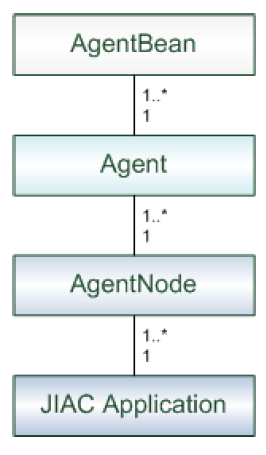
\includegraphics[width=0.25\textwidth]{images/jiac_basic.png}
		\caption{Jiac Basic concepts and their structural relationships \cite{JIACMAN10}}
	\label{fig:jiac_basic}
\end{figure}
An \textit{AgentNode} is a Java VM where the runtime infrastructure for agents, such as discovery services, white and yellow pages services, as well as communication infrastructure, are provided. A JIAC application might consists of multiple AgentNodes (distributed application). With the so-called AgentNodeBeans, one can extend the AgentNode with additional components.\\

Each AgentNode may run several \textit{Agents}. Agents provide services to other agents
and comprise lifecycle, execution cycle and a memory. An agent can use infrastructure
services in order to find other agents, to communicate to them and to use their services.
Skills and abilities of the agent can be extended by so-called AgentBeans.\\
\textit{AgentBean} is the mean to implement the functionality of an Agent, in other words, the abilities of an Agent are defined in the AgentBeans attached to it. They are plugged into agents and provide services (so-called Actions) to other agents. 

%======================================%
%                BPMN                  %
%======================================%
\section{BPMN(Business Process Modelling Notation)}
BPMN \cite{BPMN2} is a standard Notation for modelling business processes, initially published by the BPMI which is later adopted by the OMG(Object Management Group). A business process diagramm (as seen in Figure 2) can be compared to UML's activity diagram.
\begin{figure}[h]
	\centering
		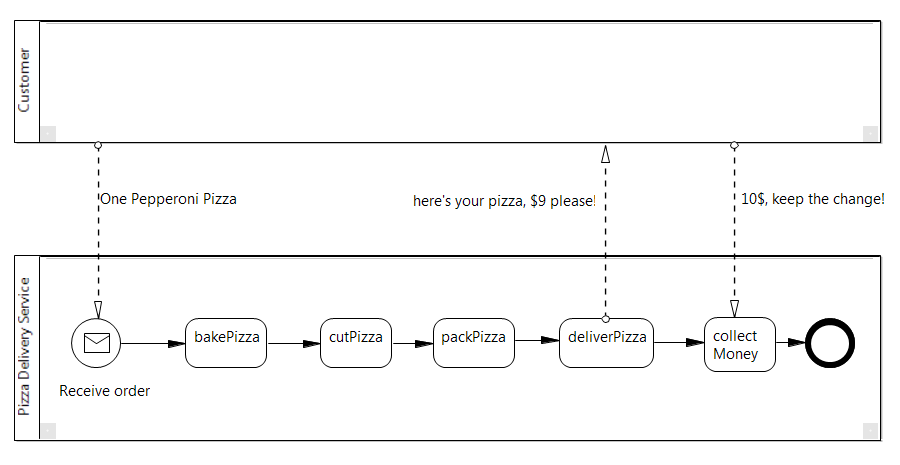
\includegraphics[width=0.90\textwidth]{images/bpmn_sampl.png}
	\caption{A simple Business Process Diagramm}
	\label{fig:bpmn_sampl}
\end{figure}\\
BPMN was made to provide a notation that is understandable by all business users, creating a brige for the gap between the business process design and the process implementation. With the mapping of BPMN to Agents, we hope to be able to increase the spreading of the multi agent systems in the business world.

BPMN elements can be categorized in five basic elements\cite{7} :
\begin{itemize}
	\item Flow Objects
	\item Data
	\item Connecting Objects
	\item Swimlanes
	\item Artifacts
\end{itemize}
\textit{Flow Objects} includes Events, Activities and Gateways. These elements are the most important in BPMN, and they are held in a lane.\\
An \textit{Event} describes something that happens during the course of a process. It is divided into Start Event, Intermediate Event and End Event (see Figure 2).
\begin{figure}[h]
	\centering
	
\includegraphics[width=0.25\textwidth]{images/events.png}
	\caption{BPMN Event types. From left to right: Start Event, Intermediate Event, End Event}
	\label{fig:events}
\end{figure}
\\
According to the type of the event's trigger(for start and intermediate events) or result(for end events), these event-types are further divided into sub-types. The event figure(see add figure) are drawn with different icon in the middle, according to it's subtype.
%=============Add figure===============%
 
An \textit{Activity} describes something that is done during a process. It is divided into \textit{Tasks} (Atomic Activities) and \textit{Sub Processes} (Composite Activities).\\
\textit{Gateways} are used to define all kinds of splitting and merging behavior. It's semantics depends on the dimension of it's incoming and outgoing Sequence Flows.
\\\\
Data is representated by the four elements:
\begin{itemize}
	\item Data Objects
	\item Data Inputs
	\item Data Outputs
	\item Data Stores
\end{itemize}
\textit{Data Object} describes information that is needed by an activity or what they produce. It can represent a singular object or a collection of objects. \textit{Data Inputs} and \textit{Data Outputs} describe the same information for Processes. \textit{Data Stores} describe the location where information, that persists beyond the scope of a process are stored.\\\\
With \textit{ConnectingObjects}, FlowingObjects can be connected to each other or with other informations. There are 3 different kinds of Connecting Objects:
\begin{itemize}
	\item \textit{Sequence Flows} - represent Flow Control, used for connecting FlowObjects within a Pool in the order of execution.
	\item \textit{Message Flows} - represent Messages being exchanged exclusively between Pools.
	\item \textit{Associations} -  mainly used for documentation, in example between Flow Objects and a Text annotation.
\end{itemize}
\textit{Swimlanes} are divided into \textit{Pools} and \textit{Lanes}. Each Pool represents one Participant in the business process, while Lanes are used to partition a Pool, in example to model different Departments of an Institution. Figure 3 shows an empty Pool with 2 Lanes.
\begin{figure}[h]
	\centering
		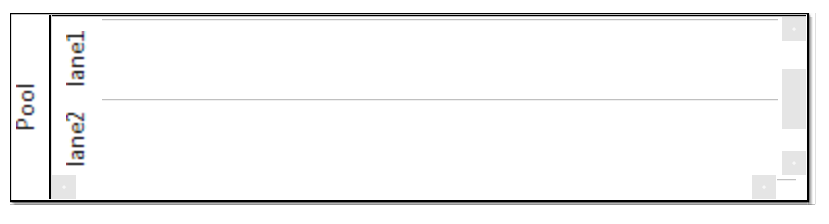
\includegraphics{images/swimlane.png}
	\caption{Empty Pool with 2 Lanes}
	\label{fig:swimlane}
\end{figure}\\\\\\
\textit{Artifacts} are additional Information about the Process. It is mainly used for documentation purpose. The Current set of Artifacts includes:
\begin{itemize}
	\item Text Annotation
	\item Group
\end{itemize}


To provide a rough overview on how Agent technology can support the implementation of Business Processes let us take a look on this mapping example of BPMN elements to Agents. A Pool in a Business Process Diagram can represent an Agent, which are able to communicate with other agents (another pool) through messages (represented with the BPMN MessageFlows). Agents can react to Events. To fully implement the transformation a detailed mapping is needed and will be developed in the scope of this work. 


%======================================%
%                VSDT                  %
%======================================%
\section{VSDT(Visual Service Design Tool)}
\label{sec:vsdt}
The VSDT is a CASE Tool, developed to support the idea of Process Oriented Agent Engineering, where Agents are designed by defining use cases and processes described with the BPMN. It's features include the BPMN editor, process structure view, model validation, import of existing web services, transformations to BPEL, and JIAC and many more. 
\begin{figure}[h]
	\centering
		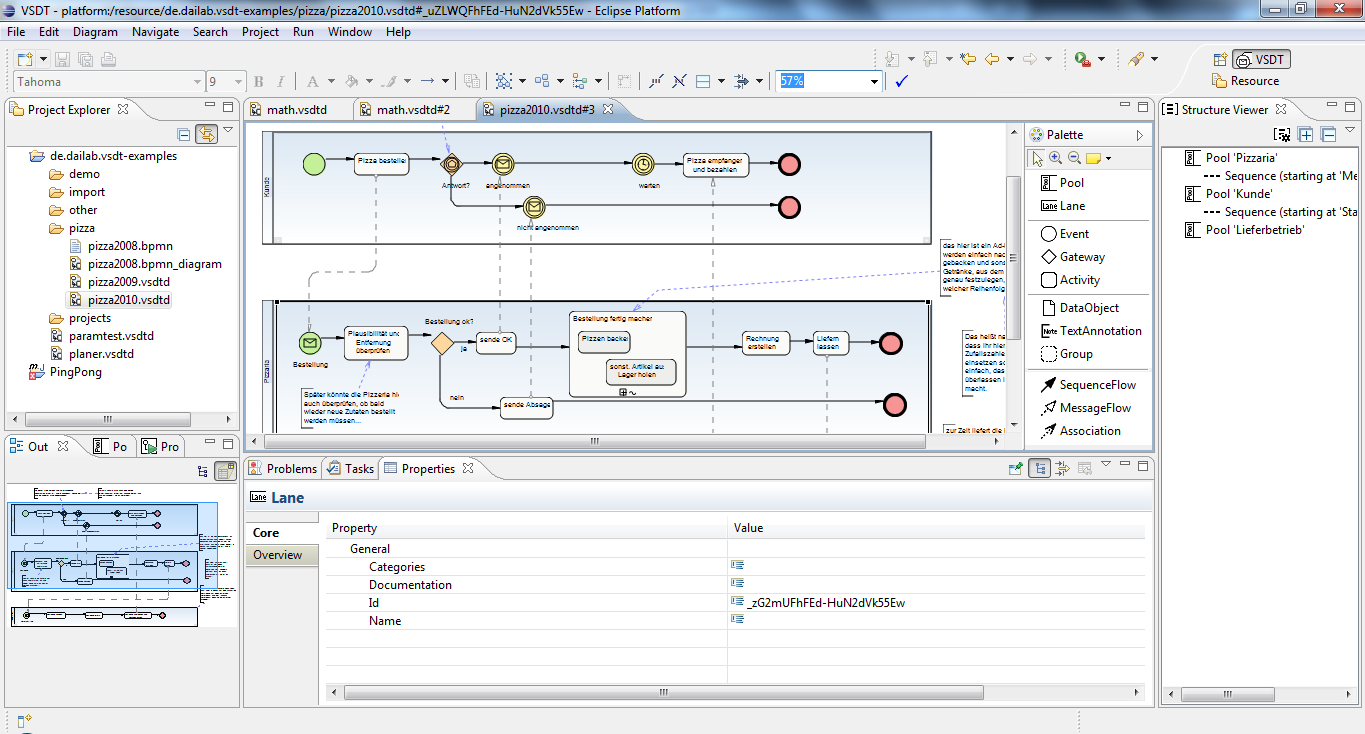
\includegraphics[width=0.90\textwidth]{images/vsdt_snapshot.png}
	\caption{VSDT - Editor View}
	\label{fig:VSDT}
\end{figure}\\

%========= The Editor =========%
\subsection{BPMN Editor}
The BPMN Editor in VSDT was created using eclipse's GMF (Graphical Modeling Framework)
%well-equipped BPMN editor that is independent of any specific target language. Thus, while the usual transformation to BPEL, as well as other transformations, is included, the VSDT can easily be extended with additional export functionality targeting other languages. It was developed in early 2007 as a Diploma Thesis at the TU Berlin and since then it has been continuously extended. 

%========= Transformation Framework ===========%
\subsection{Transformation Framework}
Since it's initial development, VSDT's transformation framework is designed to be extensible and reuseable. This allows the development of a new transformation to be easier. For this purpose the transformation process is subdivided into several stages: 
\begin{enumerate}
	\item \textit{Validation}: Validate the input model.
	\item \textit{Normalisation}: Prepare the input model for transformation.
	\item \textit{Structure Mapping}: Convert the input model to a block-like structure.
	\item \textit{Element Mapping}: Perform the actual mapping, create target model.
	\item \textit{Clean Up}: Remove redundancies, improve readability, etc.
\end{enumerate}

Due to the fact that the validation, normalisation and structure mapping are mostly independent from the target language, the standard mapping provided for these stages are reuseable, which makes it possible to implement a new transformation by specifying the element mapping only. Figure \ref{fig:transform} shows the UML Class Diagram of the transformation famework with the example transformation to BPEL.
\begin{figure}[h]
	\centering
		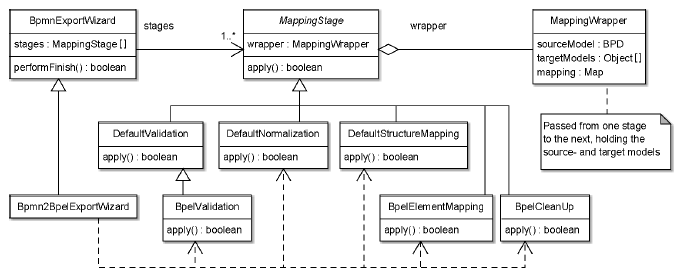
\includegraphics[width=0.90\textwidth]{images/transformation.png}
	\caption{Essential classes of the transformation framework, including the BPEL case.\cite{TK07}}
	\label{fig:transform}
\end{figure}\\

%============ Existing Transformation to Jiac ===============%
\subsection{Existing Transformation to JiacV}
At the moment, the VSDT is already equipped with a transformation of BPMN to JiacV, which generates the JADL(Jiac Agent Description Language).
The transformation to Jiac AgentBeans will be an addition to the existing transformation, as the products of both transformation has their own advantages.

\begin{tabularx}{\linewidth}{|l|X|}\hline\hline
			\multicolumn{2}{|c|}{\textbf{Advantages of:}} \\\hline
			\multicolumn{1}{|c|}{JADL} & \multicolumn{1}{c|}{AgentBeans}\\\hline
			can be deployed to a running jiac application &  Written fully in Java, therefore developer friendly.\\
																										&  Java is more powerful that JADL.\\
			                           										&  Better performance because no parser are involved.\\\hline\hline
\end{tabularx}


%======================================%
%                 JET                  %
%======================================%
\section{JET(Java Emitter Templates)}
\textit{JET}\cite{13} is a code generating framework, developed as a part of the Eclipse Modelling Project \cite{14}. JET uses templates to transform the model into any kinds of code artifacts such as java, html, xml or even plain text. \\\\
\textit{JET templates} uses a JSP-like syntax which makes it easy to write and understand. A set of JET templates is called transformation. It is possible to build this transformation with a main template which acts as a visitor and runs through the model, and this main template will then use other templates which handle a specific element of the model. For example, in UML to Java transformation you can have special templates that handles the package, class, variables and methods.\\\\

\textbf{2 different JET-Versions}\\\\
There are currently 2 different JET-Versions in the Eclipse Modelling Project. The older Version allows us to generate text with an Object as argument. In the template, one can type cast the argument variable into the class of our model. \\
The translated JET-Template will have the method \\
public String generate(Object argument)\{
...
\}

In the updated version of JET, also called JET2, some workspace and java related "'tag-libraries"' are provided, enabling us to do the transformation without using the Java and Eclipse API. Unfortunately, in this Version the model has to be an xml-File.
To directly transform the BPMN directly from it's xml-Nature will be harder and the template will be confusing, therefore a decision has been made to implement the mapping using the existing transformation framework where an intermediate model class of the AgentBean will be created, and then this intermediate model into Java code using the older version of the JET Transformation.
More details on the implementation will be discussed in chapter \ref{chap:implementation}.
	\chapter{State of the art}

%====================================================%
%                     BPMN2BPEL                      %
%====================================================%
\section{BPMN to BPEL Transformation}
In the BPMN Specification, the mapping from BPMN to BPEL has been included since the first version. In fact the development of BPMN was driven by the lack of standard notation for the WS-BPEL\cite{weidlich2008}. The limitation of the mapping from BPMN to BPEL has also been discussed in various papers, focusing the issues resulting from the incompatibility of the graph structured BPMN and the block structured BPEL, and led to some more sophisticated mapping such as the one introduced by Ouyang et al. (\cite{Ouyang2006a},\cite{Ouyang2006b}).

At the moment, there are some tools that supports the transformation from BPMN to BPEL 
In the VSDT, a mapping from BPMN to BPEL based on the mapping given in the BPMN specification was developed, covering nearly every mapping given in the specification including event handlers, inclusive OR and event based XOR Gateways. 

For this Project the mapping from BPMN to BPEL given in the BPMN specification are used to gain a better understanding of the notation's semantics.


%====================================================%
%                     BPMN2Agents                    %
%====================================================%
%======== Existing Transformation to Jiac ===========%
\section{Existing Transformation to JiacV}
At the moment, the VSDT is already equipped with a transformation of BPMN to JiacV, which generates the JADL(Jiac Agent Description Language).
As mentioned in chapter \ref{chap:background}, both JADL and AgentBean are tools to implement the functionality of an Agent in Jiac. 
The transformation to Jiac AgentBeans is in no way a replacement to the existing transformation. Instead both transformations shall complement each other as the products of both transformations have their own advantages, some of which we can find in the following table:
\begin{table}[htbp]
	\centering
		\begin{tabularx}{\linewidth}{|l|X|}\hline\hline
			\multicolumn{2}{|c|}{\textbf{Advantages of:}} \\\hline
			\multicolumn{1}{|c|}{JADL} & \multicolumn{1}{c|}{AgentBeans}\\\hline
			can be deployed to a running Jiac application &  Written fully in Java, therefore developer friendly.\\
																										&  Java is more powerful that JADL.\\
			                           										&  Better performance because no parser are involved.\\\hline\hline
		\end{tabularx}
\end{table}

\newpage
\section{WADE}
A similar approach (designing agents behavior with processes and transforming it into Java Code) has been developed by the Telecom Italia with their JADE-extension called WADE (Workflows and Agents Development Environment). While Jade was developed to simplify the implementation of Software Agents, WADE extended JADE with a workflow engine, making it possible to create Agents that executes tasks defined as workflows.

\subsection{JADE (\textbf{J}ava \textbf{A}gent \textbf{DE}velopment Frameork)}
JADE (\cite{FBGCAPGR08},\cite{FBAPGR99}) is an application framework and a middleware written in Java, which support the development of software agents. The framework  provides distributed runtime environments, agent and behaviour abstractions as well as communications between agents and discovery mechanisms. We can say that it's role is very similar to JIAC.

\subsection{WADE (Workflows and Agents Development Environment)}
WADE is an extension to JADE, which enrich the application framework with a workflow engine. The WorkflowEngineAgent extends the JADE basic Agent class with an ability to execute workflows represented in a WADE specific formalism.

A WADE workflow is actually a Java Class, thus it can be edited and managed as Java classes and can contain pieces of code which is needed to implement the process. With WOLF, a development environment that comes with WADE, developers can edit the Workflow graphically as well as textually. The code view and the graphical view of the workflow are kept in sync.

Despite having all the advantages of a Java code, the WADE workflow is rather simple and not so expressive as the BPMN. Similarity to the agent technology such as event handling and communication flow are also missing in the workflow. In the following we will take a closer look on the workflow concept of Wade. 


\subsection{Workflow Metamodel (graphical view)}
For the graphical view of the workflow, WADE adopts a workflow metamodel quite similar to that defined in XPDL standard defined by the Workflow Management Consortium (www.wfmc.org). In figure \ref{fig:wade_elements} (image taken from \cite{GCDGMB08}), we can see an example process summarizing the main elements of the WADE metamodel.
\begin{figure}[h]
	\centering
		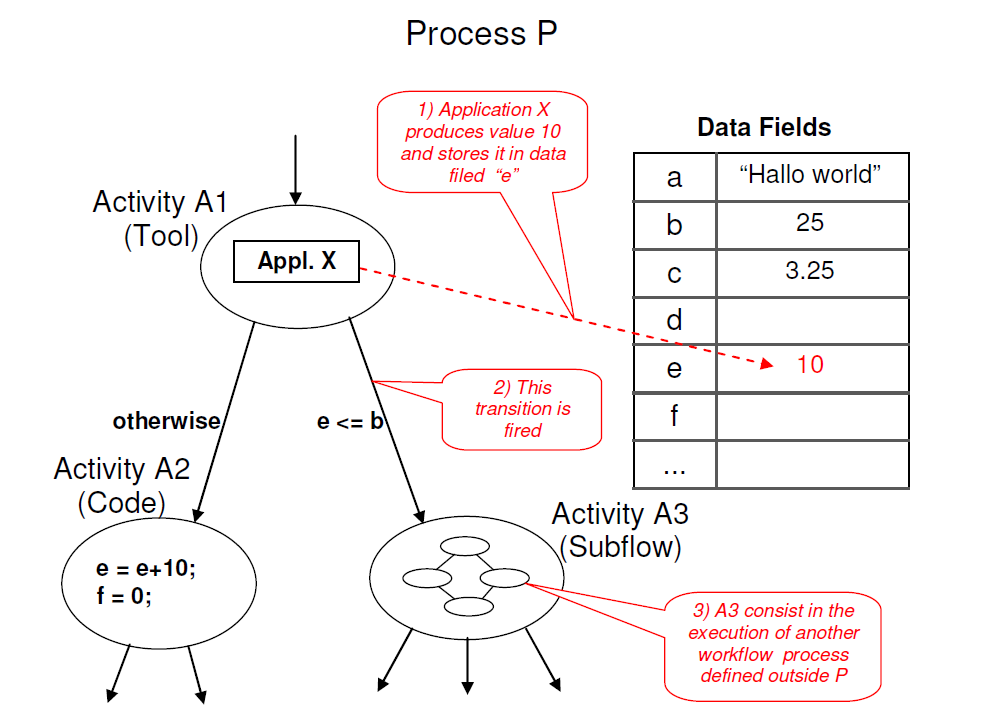
\includegraphics[width=1.00\textwidth]{images/wade_elements.png}
	\caption{Elements of Wade Metamodel \cite{GCDGMB08}}
	\label{fig:wade_elements}
\end{figure}

A Process in Wade is made up from a set of Activities, where each activity corresponds to the execution of the given operations. A Process is defined with exactly one \textbf{Start Activity}, and one or multiple \textbf{End Activities}. A Process may have Formal Parameters, which defines the type of required inputs and expected outputs.

Activities in Wade are divided into different types depending on the operations included in the activity. 6 types are mentioned in \cite{GCWADEUG10} as being the most relevant:
\begin{itemize}
	\item \textbf{\textit{Tool Activities}}\\
	      Contains the invocation of one or more \textbf{Applications}, computational entities defined outside of the workflow process and wrapped by a uniform interface.
	\item \textbf{\textit{Subflow Activities}}\\
	      Contains the invocation of another workflow process. The execution of the subflow takes place in a different computational place and it may be carried out by another agent. Further, we can set whether the subflow should be executed synchronously or asynchronously.
	\item \textbf{\textit{Webservice Activities}}\\
				Contains the invocation of a webservice.
	\item \textbf{\textit{Code Activities}}\\
				Included operations are specified directly by a set of Java code. 
	\item \textbf{\textit{Subflow Join}} \\
	      Included operations consist of blocking the main workflow process and wait untill the previously launched asynchronous subflow completes, and getting the results.
	\item \textbf{\textit{Route Activities}}\\
				Route activities are empty. No operations is included. It can be used to simplify complex flows. 
\end{itemize}
% explain the Wade-Workflow, add screnshots etc.
Each non ending activity has one or more outgoing \textbf{\textit{Transitions}} leading to another activity. A transition may be associated with a condition. Once an activity completes, the conditions of all outgoing transitions will be checked. If the condition holds, the transition will be fired and the workflow continues with the execution of the destination activity.

A Process has a set of \textbf{DataFields} which can be referenced anywhere in the process e.g. in the condition of a transaction or in the operations included in an activity. 
\\\\

\subsection{Workflow implementation (code view)}
As mentioned before, workflow in wade is actually a (well structured) Java class. A workflow process is implemented by a Java class extending the \verb|WorkflowBehaviour| class, which provides the methods \verb|registerActivity()| and \verb|registerTransition()| for adding activities and transitions into the process. 

The \verb|registerActivity()| method takes a behaviour object as argument. There are different behaviour classes corresponding to the different activity types discussed in the previous subsection. The actual operations included for the registered activity are wrapped in a void method of the workflow class. The method's name is derived from the activity's name added with the ''execute'' prefix e.g \verb|executecheckBalance()| for the activity ''checkBalance''.  

The \verb|registerTransition()| method takes a Transition object as an argument. If the transition is associated with a condition, then a boolean method (with the prefix ''check'' added to the condition name) will be created.

In Figure \ref{fig:wade_graph} we can see an example process in its graphical view and Listing \ref{list:wade_code} shows the equivalent code view to the example. 

\begin{figure}[h]
		\centering
		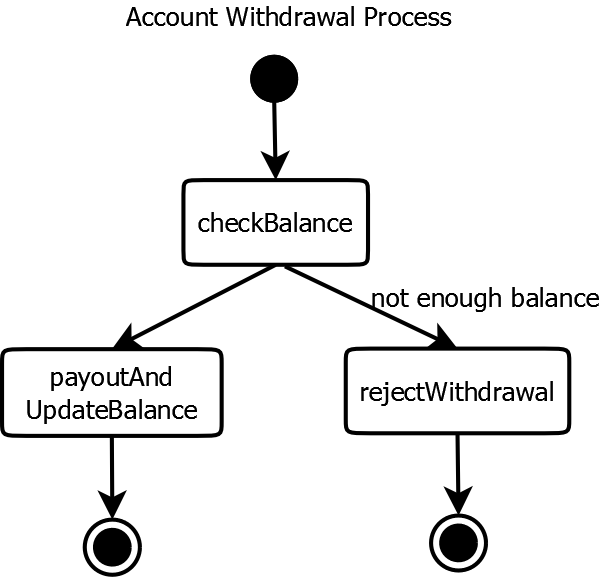
\includegraphics[width=0.5\textwidth]{images/wade_example.png}
		\caption{Wade example: Account Withdrawal Process (graphical view)}
	  \label{fig:wade_graph}
\end{figure}
\newpage
\begin{lstlisting}[language = Java, caption=Wade example: Account Withdrawal Process (code view), label = list:wade_code]
//the layout information of the graphical view
@WorkflowLayout(entryPoint = @MarkerLayout(position = "(260,31)", activityName = "checkBalance"), exitPoints = { }, transitions = {@TransitionLayout(to = "rejectWithdrawal", from = "checkBalance"), @TransitionLayout(to = "payoutAndUpdateBalance", from = "checkBalance") }, activities = {@ActivityLayout(position = "(357,175)", name = "rejectWithdrawal"), @ActivityLayout(position = "(116,171)", name = "payoutAndUpdateBalance"), @ActivityLayout(position = "(222,78)", name = "checkBalance") })

public class AccountWithdrawal extends WorkflowBehaviour {
	//Data fields
	public static final String NOTENOUGHBALANCE_CONDITION = "notEnoughBalance";
	public static final String REJECTWITHDRAWAL_ACTIVITY = "rejectWithdrawal";
	public static final String PAYOUTANDUPDATEBALANCE_ACTIVITY = "payoutAndUpdateBalance";
	public static final String CHECKBALANCE_ACTIVITY = "checkBalance";
	private double balance;
	
	//formal Parameter
	@FormalParameter(mode=FormalParameter.INPUT)
	public double amountToBeWithdrawn;
	
	// All activities should be registered in this method
	private void defineActivities() {
		CodeExecutionBehaviour checkBalanceActivity = new CodeExecutionBehaviour(
				CHECKBALANCE_ACTIVITY, this);
		registerActivity(checkBalanceActivity, INITIAL);
		CodeExecutionBehaviour payoutAndUpdateBalanceActivity = new CodeExecutionBehaviour(
				PAYOUTANDUPDATEBALANCE_ACTIVITY, this);
		registerActivity(payoutAndUpdateBalanceActivity, FINAL);
		CodeExecutionBehaviour rejectWithdrawalActivity = new CodeExecutionBehaviour(
				REJECTWITHDRAWAL_ACTIVITY, this);
		registerActivity(rejectWithdrawalActivity, FINAL);
	}

	// All transitions should be registered here
	private void defineTransitions() {
		registerTransition(new Transition(), CHECKBALANCE_ACTIVITY,
				PAYOUTANDUPDATEBALANCE_ACTIVITY);
		registerTransition(new Transition(NOTENOUGHBALANCE_CONDITION, this),
				CHECKBALANCE_ACTIVITY, REJECTWITHDRAWAL_ACTIVITY);
	}

  //activity methods
	protected void executecheckBalance() throws Exception {
		[code for checking the account's balance]
	}

	protected void executepayoutAndUpdateBalance() throws Exception {
	  [...]
	}

	protected void executerejectWithdrawal() throws Exception {
		[...]
	}

	//check method for the condition of a transition
	protected boolean checknotEnoughBalance() throws Exception {
		return true;
	}

}
\end{lstlisting}

From the above listing, we can see the structure of a workflow implementation class in Wade. At line 3, we can see how the layout information for the graphical view is coded with the Java annotation mechanism. Data fields are implemented as a class variable (line 6-10) so that it can be referenced everywhere in the workflow process. 

Although it is not strictly necessary, all activities and transitions should be registered in the methods \verb|defineActivities()| and \verb|defineTransitions()| because the graphical editor will search these methods to detect the activities and transitions to show.

In line 38 to 47 we can see the activity methods that wraps the operations included in an activity. And finally we can see the boolean method  \verb|checknotEnoughBalance()| that checks for the condition of the transition from checkBalance to rejectWithdrawal. These methods are per default empty, leaving the operations to be added directly into the code by the developer.

Wade's approach in implementing the workflow as Java code has inspired us for this project. Some of the concepts e.g wrapping the activity in a java method can also be found in our BPMN to AgentBean transformation. 
	%concept von wade nach bpmn2jiacbeans
	\chapter{Mapping BPMN to Jiac AgentBeans}
\label{chap:mapping}
The element mapping from BPMN to Jiac AgentBeans is created based on the existing mapping to JiacV - JADL script. Compared to a JADL script, an AgentBean that is written completely in Java enables more possibilities in mapping concepts such as intermediate Event handling. Some concepts found in Wade's workflow implementation inspired us for the development of the mapping. This chapter will provide a detailed overview of the mapping.\\\\

%%%%%%%%%%%%%%%%%%%%%%%%%%%%%%%%%%%%%%%%%%%%%%%%%%%%%%%
% 4.1 Pools & Processes                               %
%%%%%%%%%%%%%%%%%%%%%%%%%%%%%%%%%%%%%%%%%%%%%%%%%%%%%%%
\section{Pools and Processes}
Every pool in a process diagram will be mapped into an AgentBean. The name of the AgentBean will be derived from the Pool name, and the name of the process diagram it is contained in. If a Pool with the same name (e.g Mathematican) is contained in the business process diagrams ExtractRoot and Faculty, then the two agent beans \texttt{Mathematican\_ExtractRoot} and \texttt{Mathematican\_Faculty} will be created. Further, they are grouped in the package mathematican. 

The process contained in a pool is mapped into a \textbf{workflow method}. Depending on the start event's type, this workflow method may be called in the execute method of the bean (for timer start event), it may be exposed as an action (for message start event with service implementation), or if the start event is a message start event with MessageChannel implementation, a SpaceObserver will be created and attached to the agent's memory, which will call the workflow method when a message with the payload and address as specified in the implementing message channel are written into the agent's memory.

The mapping of a task contained in a process flow will be wrapped in the so called \textbf{activity method} which will be called by the workflow method. Special cases for tasks with event handler and subprocesses will be discussed in a later section.

Lanes are currently ignored. A process of a lane will be handled as a process of the containing pool.

\begin{figure}[h]
	\centering
		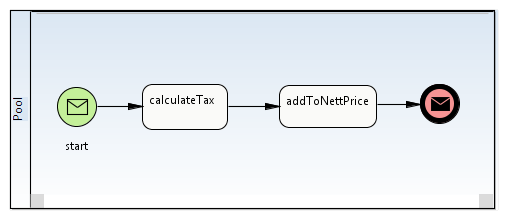
\includegraphics[width=0.80\textwidth]{images/mapping/pool_and_process.png}
	\caption{Mapping example : Pool and Process}
	\label{fig:pool+process}
\end{figure}

The Figure\ref{fig:pool+process} shows a simple example of a pool called Pool with the process doProcess. For the Pool, a Java class called Pool\_DoProcess will be created and it will have the workflow method called doProcess. In this example the message start event is implemented as a service, thus the workflow method is exposed as an Action as we can see in the following Listing \ref{list:pool+process}.  
\begin{lstlisting}[language = Java, caption =  Mapped element: Pool and Process (Figure \ref{fig:pool+process}), label = list:pool+process]
package pool;//derived from the pool name

//some imports...

public class Accounting_CalculatePrice extends AbstractMethodExposingBean{
	
	public final static String ACTION_DOPROCESS = "pool.Pool_DoProcess#doProcess"; 
	
	// process attribute would be declared here
	[...]
	@Expose(name = ACTION_DOPROCESS, scope = ActionScope.GLOBAL)
	public double doProcess(double nettPrice, double taxRateInPercent) {
		calculateTax();
		addToNettPrice();
		return totalPrice;
	}
	
	private void calculateTax(){
		[...]
	}
	
	private void addToNettPrice(){
		[...]
	}
}
\end{lstlisting}


\section{Workflow Structure}
Workflow structure is mapped as the content of the workflow method. It defines the invocation structure of the flow objects contained in a process.

\subsection{Sequence Flow}
The mapping of a sequence flow is trivial. The mapped elements connected with a sequence flow will be invoked sequentially in the workflow method (see Figure \ref{fig:mapping_sequence}).\\

\begin{figure}[h]
\begin{minipage}[c]{0.5\textwidth}
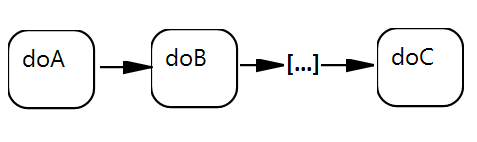
\includegraphics[width=0.9\textwidth]{images/mapping/sequence.png}
\end{minipage}
\begin{minipage}[c]{0.5\textwidth}
\begin{lstlisting}[language=Java]
doA();
doB();
[...]
doC();
\end{lstlisting}
\end{minipage}
\caption{Mapping Example: Sequence Flow}%
\label{fig:mapping_sequence}%
\end{figure}

\subsection{Gateways}
Branches of a gateway are wrapped according to the gateway's type. There are 5 different types of gateways:
\begin{enumerate}
	\item AND (Parallel)
	\item OR (Inclusive)
	\item XOR\_Data (Exclusive)
	\item XOR\_Event (Event Based)
	\item Complex 
\end{enumerate}

%%%%%%%%%%%%%%%%%%%%%%%%%%%%%%%%%%%
\textbf{AND-Gateway (Parallel)}\\
In an AND-Gateway, all branch will be wrapped in parallel to one another. At runtime all branches are executed within a thread. 
Figure \ref{fig:mapping_AND} shows an example of the mapping. \\

\begin{figure}[h]%
\begin{minipage}[c]{0.5\textwidth} 
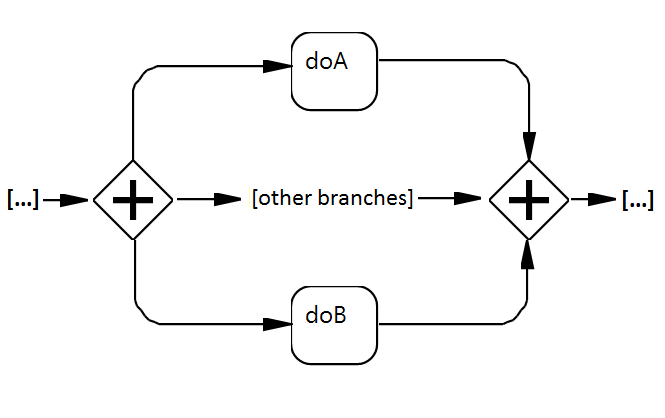
\includegraphics[width=0.95\linewidth]{images/mapping/and-gateway.png}
\end{minipage}
\begin{minipage}[c]{0.5\textwidth} 
\begin{lstlisting}[language=Java]
[...]
Thread and_branch1 = new Thread(){
	public void run(){
		doA();
	}
};
[create thread for other branches]
Thread and_branch2 = new Thread(){
	public void run(){
		doB();
	}
};
and_branch1.start();
[start other branches]
and_branch2.start();
try {
	and_branch1.join();
	[join other branches]
	and_branch2.join();
} catch(InterruptedException) { }
[...]
\end{lstlisting}
\end{minipage}
\caption{Mapping example: AND Gateway}%
\label{fig:mapping_AND}%
\end{figure}



%%%%%%%%%%%%%%%%%%%%%%%%%%%%%%%%%%%%%
\textbf{OR-Gateway (Inclusive)}\\
Branches of an OR-Gateway will also be executed in parallel to one another, but the content of a branch is additionally wrapped in an if-then block as shown in Figure \ref{fig:mapping_OR}. At runtime, the condition of each branches will be checked and the branch will be skipped if the condition does not hold. However, if the or-gateway has a branch with default condition, the default branch will only be executed if none of the other branches are executed.
\begin{figure}[h]
\begin{minipage}[c]{0.5\textwidth}
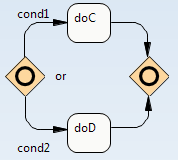
\includegraphics[width=0.95\textwidth]{images/mapping/or-gateway.png}
\end{minipage}
\begin{minipage}[c]{0.5\textwidth}
\begin{lstlisting}[language=Java]
[...]
Thread or_branch1 = new Thread(){
	public void run(){
		if(cond1){
			doA();
		}
	}
};
[thread for other branches]
Thread or_branch2 = new Thread(){
	public void run(){
		if(cond2){
			doB();
		}
	}
};
or_branch1.start();
[start other branches]
or_branch2.start();
try {
	or_branch1.join();
	[join other branches]
	or_branch2.join();
} catch(InterruptedException) { }
[...]
\end{lstlisting}
\end{minipage}
\caption{Mapping example: OR Gateway}%
\label{fig:mapping_OR}%
\end{figure}


\textbf{XOR\_Data-Gateway (Exclusive)}\\
Branches of an XOR\_Data are wrapped in an if-then-else block (see Figure \ref{fig:mapping_xorData}). Only one branch will actually be executed at runtime. \\

\begin{figure}[h]
\begin{minipage}[c]{0.5\textwidth}
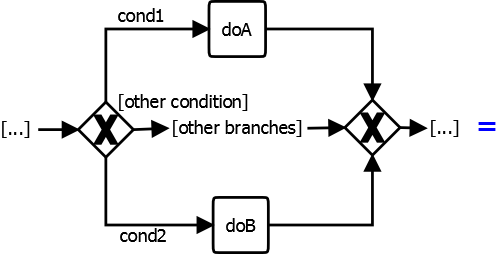
\includegraphics[width=0.95\textwidth]{images/mapping/xor-data.png}
\end{minipage}
\begin{minipage}[c]{0.5\textwidth}
\begin{lstlisting}[language=Java]
[...]
if(cond1){
	doA();
}else{
	if([other condition]){
		[other branches]
	}else{
		if(cond2){
			doB();
		}
	}
[...]
\end{lstlisting}
\end{minipage}
\caption{Mapping example: XOR\_Data Gateway}%
\label{fig:mapping_xorData}%
\end{figure}

\textbf{XOR\_Event-Gateway (Event Based)}\\
For XOR\_Event, a waiting loop will be started in a Thread, and an EventHandler (an extension to java.lang.Thread) instance for each branch will be created and started, according to the event's trigger of each branch. If an event handler receive an event, the waiting thread will be stopped, and the process continues with the elements of the branch, and other branches will be skipped. Figure \ref{fig:mapping_xorEvent} shows an example of the mapping.

\begin{figure}[h]
\begin{minipage}[c]{0.5\textwidth}
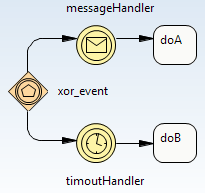
\includegraphics[width=0.9\textwidth]{images/mapping/xor-event.png}
\end{minipage}
\begin{minipage}[c]{0.5\textwidth}
\begin{lstlisting}[language=Java]
[...]
Thread xor_event_wait = new Thread(){
	public void run() {
		while(true) {
			try {
				Thread.sleep(100);
			} catch(InterruptedException e) {}
		}
	}
};
MessageEventHandler messageHandler = new MessageEventHandler(xor_event_wait);
[handler for other branches]
TimeoutEventHandler timeoutHandler = new TimeoutEventHandler(20000, xor_event_wait);
//start the wait activity and all handlers
xor_event_wait.start();
messageHandler.start();
[start other handlers]
timeoutHandler.start();
try{
	xor_event_wait.join();
	timeoutHandler.stop();
	[stop other handlers]
	messageHandler.stop();
} catch (InterruptedException e) {
	if(messageHandler.hasBeenTriggered()){
		doA();
	}
	[other branches]
	if(timeoutHandler.hasBeenTriggered()){
		doB();
	}
}
[...]
\end{lstlisting}
\end{minipage}
\caption{Mapping example: XOR\_Event Gateway}%
\label{fig:mapping_xorEvent}%
\end{figure}
\newpage
The event handler class will be added as an inner class to the bean, and they will have a constructor with a Thread toStop argument (among other arguments) and a boolean method \verb|hasBeenTrigerred()| to check whether the event handler has been activated by the expected event. The following Listing \ref{list:timeoutEventHandler} shows an implementation of the TimeoutEventHandler. This inner class will be included in every agent bean class that uses a TimeoutEventHandler.\\\\

\begin{lstlisting}[language=Java, caption=TimeoutEventHandler implementation as an inner class, label=list:timeoutEventHandler]
class TimeoutEventHandler extends Thread{
		
		long timeout;
		Thread toStop;
		boolean triggered = false;
		
		public TimeoutEventHandler(long timeout, Thread toStop){
			this.timeout = timeout;
			this.toStop = toStop;
		}
		
		public void run(){
			try {
				Thread.sleep(timeout);
				triggered = true;
				toStop.stop();
			}catch(InterruptedException e ) { }
		}
		
		public boolean hasBeenTriggered(){
			return triggered;
		}
		
}
\end{lstlisting}

\textbf{Complex-Gateway}\\
A mapping concept for Complex Gateways has not been developed in the current Version. \\

\subsection{Loop Blocks}
Structured loop blocks are mapped as shown in Figure \ref{fig:mapping_loop}.
\begin{figure}[h]
\begin{minipage}[c]{0.5\textwidth}
	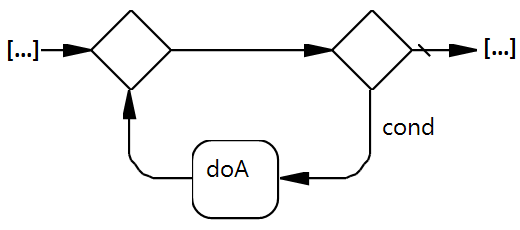
\includegraphics[width=0.95\textwidth]{images/mapping/loop_block.png}
\end{minipage}
\begin{minipage}[c]{0.5\textwidth}
\begin{lstlisting}[language=Java]
[...]

while(cond){
	doA();
}

[...]
\end{lstlisting}
\end{minipage}
\caption{Mapping example: Loop Blocks }%
\label{fig:mapping_loop}%
\end{figure}

While the condition applies, the content branch will be repeated. 

\begin{figure}[h]
\begin{minipage}[c]{0.45\textwidth}
	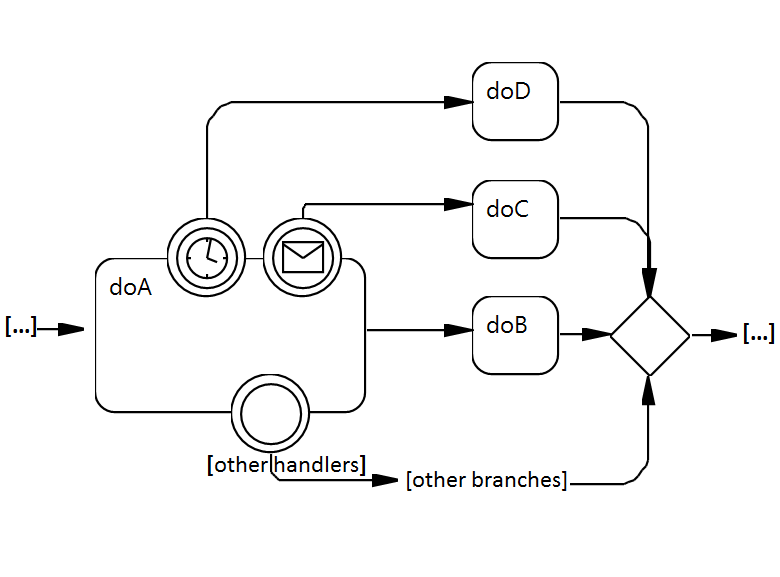
\includegraphics[width=0.95\textwidth]{images/mapping/event_handler.png}
\end{minipage}
\begin{minipage}[c]{0.55\textwidth}
\begin{lstlisting}[language=Java]
[...]
Thread doA_Thread = new Thread(){
	public void run(){
		doA();
	}
};
MessageEventHandler messageHandler = new MessageEventHandler(doA_Thread);
TimeoutEventHandler timeoutHandler = new TimeoutEventHandler(20000, doA_Thread);
[other handlers]

doA_Thread.start();
messageHandler.start();
timeoutHandler.start();
[start other handlers]

try{
	doA_Thread.join();
	timeoutHandler.stop();
	messageHandler.stop();
	[stop other handlers]
} catch(InterruptedException e) {
	if(messageHandler.hasBeenTriggered(){
		doC();
	}
	if(timeoutHandler.hasBeenTriggered(){
		doD();
	}
	if([other handlers].hasBeenTriggered()){
		[...]
	}
}

//doB only if none of the 
//event handlers are triggered
if(!messageHandler.hasBeenTriggered()){
	if(!timeoutHandler.hasBeenTriggered()){
		if(![other handlers].hasBeenTriggered()){	
			doB(); 
		}
	}
}

[...]
\end{lstlisting}
\end{minipage}
\caption{Mapping example: Event Handler}%
\label{fig:mapping_eventhandler}%
\end{figure}

\subsection{Event Handler}
As we can see in Figure \ref{fig:mapping_eventhandler}, the mapping of an Event Handler attached to an activity is somewhat similar to the mapping of gateway event. Instead of the waiting thread, a thread calling the activity method will be created, and it will be stopped if the event handler is triggered.\\

\newpage
\section{Activites}
Now we will discuss the activities in details. Activities are divided into tasks and subprocess. As mentioned before, a task will be wrapped in an activity method. This enables each task to have their own scope of properties. The properties of subprocesses however, should be shared with all activities contained in it. Therefore wrapping subprocesses in a method is not enough. Instead a subprocess will be wrapped in an inner class.
 
\subsection{Tasks}
Basically, the activity method generated from a task will look like what we can see in Figure \ref{fig:mapping_task}:

\begin{figure}[h]
\begin{minipage}[c]{0.3\textwidth}
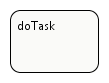
\includegraphics[width=0.95\textwidth]{images/mapping/task.png}
\end{minipage}
\begin{minipage}[c]{0.7\textwidth}
\begin{lstlisting}[language=Java]
public void doTask(){
	[declaration of properties]
	[start assignments]
	[special mapping depending on task-type]
	[end assignments]
}
\end{lstlisting}
\end{minipage}
\caption{Mapping example: Task}%
\label{fig:mapping_task}%
\end{figure}
\newpage
The method will start by declaring java variables, derived from the task's properties (if any exists). After the declaration, start assignments will take place, followed by the task's actual mapping (if any, depending on the task type). Finnaly, the code will be closed with the end assignments. The BPMN allows us to specify properties and assignments (including when the assignment should take place) in the task's property sheet. Thus, other than the workflow model in Wade, it is possible to generate the operations needed to execute the activity completely from the model. Now let's take a closer look on how specific task types are being mapped.\\

\textbf{Script-task}\\
For Script-tasks, the script defined in the task's property will be directly added into the activity-method. This type of task is comparable to Wade's \textit{Code Activity}, but just like the properties and assignments, with BPMN the script can be specified in the property sheet of the task. For the transformation to agent beans, the given script should be a valid Java expression. \\\\


\textbf{Service-task}\\
A service task is mapped into an invocation of an Action defined by other Bean.\\

\begin{figure}[h]
\begin{minipage}[c]{0.3\textwidth}
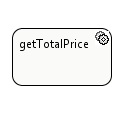
\includegraphics[width=0.95\textwidth]{images/mapping/service_task.png}
\end{minipage}
\begin{minipage}[c]{0.7\textwidth}
\begin{lstlisting}[language=Java]
[...]
Action [operation] = retrieveAction([interface].[operation]);
Serializeable [] results = invokeAndWaitForResults([operation], new Serializeable[]{[inputs]}).getResults();
[assign outputs from results]
[...]
\end{lstlisting}
\end{minipage}
\caption{Mapping example: Service-task}%
\label{fig:service_task}%
\end{figure}
Figure \ref{fig:service_task} shows how a service task would be mapped. First, the action has to be found. Then the service will be invoked and the result will be assign to the outputs defined in the task's implementing Service.\\\\

\textbf{Send-task}\\
A Send task will be mapped into an invocation of the ICommunicationBean's send action (see Figure \ref{fig:send_task}). The group address, to which the message should be sent, and the message itself will be derived from the given MessageChannel in the task's properties. \\\\
 
\begin{figure}[h]
\begin{minipage}[c]{0.3\textwidth}
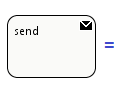
\includegraphics[width=0.95\textwidth]{images/mapping/sendTask.png}
\end{minipage}
\begin{minipage}[c]{0.7\textwidth}
\begin{lstlisting}[language=Java]
[...]
Action sendAction = retrieveAction(ICommunicationBean.ACTION_SEND);
IGroupAddress groupAddress = CommunicationAddressFactory.createGroupAddress([address]);
JiacMessage jiacMessage = new JiacMessage([payload]);
invoke(sendAction, new Serializable[]{jiacMessage, groupAddress});
[...]
\end{lstlisting}
\end{minipage}
\caption{Mapping example: Send-task}%
\label{fig:send_task}%
\end{figure}


\textbf{receive-task}\\
A receive-task will be mapped into a Java-Code that reads the memory and wait until the specified message defined by the given MessageChannel is found in the memory. \\

\begin{figure}[h]
\begin{minipage}[c]{0.3\textwidth}
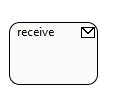
\includegraphics[width=0.95\textwidth]{images/mapping/receiveTask.png}
\end{minipage}
\begin{minipage}[c]{0.7\textwidth}
\begin{lstlisting}[language=Java]
[...]
Action joinAction = retrieveAction(ICommunicationBean.ACTION_JOIN_GROUP);
Action leaveAction = retrieveAction(ICommunicationBean.ACTION_LEAVE_GROUP);
IGroupAddress groupAddress = CommunicationAddressFactory.createGroupAddress([address]);
invoke(joinAction,new Serializable[]{groupAddress});
[payload] = null;
while([payload name]==null) {
	Set<IFact> all = memory.readAll();
	for(IFact fact : all){
		if(fact instanceof JiacMessage) {
			JiacMessage jiacMessage = (JiacMessage)fact;
			if(jiacMessage.getPayload() instanceof Ping && jiacMessage.getHeader(IJiacMessage.Header.SEND_TO).equals(groupAddress)) {
				memory.remove(jiacMessage);
				[payload name] = ([payload type]) jiacMessage.getPayload();
				break;
			}
		}
	}
	try{
		Thread.sleep(100);
	} catch(InterruptedException e) { }
}
invoke(leaveAction, new Serializable[]{groupAddress});
[...]
\end{lstlisting}
\end{minipage}
\caption{Mapping example: receive-task}%
\label{fig:receive_task}%
\end{figure}

\textbf{Call-task}\\
A call task will be mapped to an invocation of the called element. If the called element is an activity, then the activity method will be called. 
If the called element is a Pool, then the call task will be mapped into a service invocation. 

\textbf{User task}\\
The mapping of user tasks has not been completely developed yet. User tasks requires a User Interface module to get inputs from the user. To make it simple we can put a TODO flag in the code, and the developer should implement the UI manually. 

\textbf{Manual task}\\
Manual tasks won't be executed manually, therefore a mapping won't be needed.

\textbf{BusinessRule-tasks}\\
The mapping of business rule tasks doesn't exist in this Version.

\subsection{Subprocess}
A subprocess will be mapped into an inner class of the containing Process or Subprocess. This way it's properties can be shared among all tasks contained in it. The inner subprocess will have the method \texttt{public void run()} containing the workflow (similar to the bean's workflow method). The following example shows the mapping of a subprocess:\\

\begin{figure}[h]
\begin{minipage}[c]{0.3\textwidth}
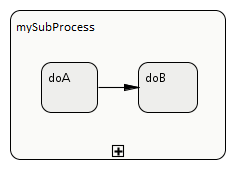
\includegraphics[width=0.95\textwidth]{images/mapping/subprocess.png}
\end{minipage}
\begin{minipage}[c]{0.7\textwidth}
\begin{lstlisting}[language=Java]
//workflow-method
public void doProcess{
[...]
MySubProcess mySubProcess = new MySubProcess();
mysubProcess.run();
[...]
}

[...]
// subprocess as Innerclass
class MySubProcess {
	[declaration of properties]
		
	public void run(){
		doA();
		doB();
	}
	
	private void doA(){
		[...] 
	}
	
	private void doB(){ 
		[...] 
	}
}
\end{lstlisting}
\end{minipage}
\caption{Mapping example : Subprocess}%
\label{fig:mapping_subprocess}%
\end{figure}

\subsection{Activity-Looping}
An activity can have a looping property. This will result in the wrapping of the task-specific mapping in a while-block. 
There are two types of activity-looping in BPMN:
\begin{enumerate}
	\item Standard-Loop
	\item Multi Instance Loop
\end{enumerate}
While the mapping of a standard-loop is trivial, the semantics of the multi instance loop is not very clear. Thus, a mapping of multi instance loop is not yet included in this version.
 
\textbf{Standard-Loop}
In a standard loop, the task specific mapping will be wrapped in a while block. The other elements of the activity method (variable declarations and assignments) will not be wrapped.  In Figure \ref{fig:mapping_standardLoop} we can see an example of a script task with a standard loop.
\begin{figure}[h]
\begin{minipage}[c]{0.3\textwidth}
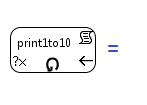
\includegraphics[width=0.95\textwidth]{images/mapping/standard_loop.png}
\end{minipage}
\begin{minipage}[c]{0.7\textwidth}
\begin{lstlisting}[language=Java]
public void print1To10(){
	int index;
	[more variable declarations]
	index= 1;
	[more start assignments]
	while((index < 11)) {
		System.out.println(index++);
	}
	[end assignments]
}
\end{lstlisting}
\end{minipage}
\caption{Mapping example : Activity-Looping (Standard Loop)}% 
\label{fig:mapping_standardLoop}%
\end{figure}

\section{Events}
Finally, we will now discuss the mapping of BPMN Events to Jiac AgentBeans. We will first discuss the Intermediate events and then we will handle Start and End Events. We need to group start and end events because the mapping will have influence on how the process will be started, and they will also determine the signature (input and output parameters) of the workflow method. 

\subsection{Intermediate-Events}
Intermediate Events are something that happens during the process. It's mapping will be added into the workflow method. To keep the workflow method readable, we decided to wrap intermediate events in a method (similar to activities). The name will be derived from the events name (if specified) or id, added with an event-type specific postfix.

In this version only the mapping of Timer and Message intermediate events are included. 

\textbf{Timer}\\
A timer intermediate event will turn the process to sleep until the given time expression. If the given time expression is a duration (option as duration in the property sheet is selected), then the expression will be handled as a long integer that defines how long (in milliseconds) the process should be paused.\\

If the given time is an exact time (e.g. Friday, November 4th 2011 10:00:00), then the expression should be parsed into a Java Date object and the process should be paused until the given date. However, it is not clear yet on how to handle incomplete date expressions (e.g. when we need to start a process every day at midnight). At the moment, the given date expression has to be in the form ''yyyy-MM-dd'T'HH:mm:ss.SSSZ'' (e.g. 2011-11-04T10:00:00.000+0100 for Friday, November 4th 2011 10:00:00). Figure \ref{fig:timer_intermediate}
shows an example of the mapping for both variants.
\begin{figure}[h]
\begin{minipage}[c]{0.28\textwidth}
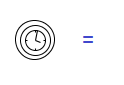
\includegraphics{images/mapping/timer_intermediate.png}
\end{minipage}
\begin{minipage}[c]{0.72\textwidth}
If the expression is a duration:
\begin{lstlisting}[language = Java]
[...]
try {
	Thread.sleep([time expression]);
} catch(InterruptedException e) {
}
[...]
\end{lstlisting}
If the expression is an exact time:
\begin{lstlisting}[language = Java]
[...]
try {
Date then = new SimpleDateFormat("yyyy-MM-dd'T'HH:mm:ss.SSSZ").parse([time expression]);
long toSleep = then.getTime() - System.currentTimeMillis();
if(toSleep>0){
	try {
		Thread.sleep(toSleep);
	} catch(InterruptedException e) {
	}
}
} catch(ParseException e) {
	System.out.println("ParseException: Time has to be in yyyy-MM-dd'T'HH:mm:ss.SSSZ form");
	e.printStackTrace();
}
[...]
\end{lstlisting}
\end{minipage}
\caption{Mapping example : Timer Intermediate Event}%
\label{fig:timer_intermediate}%
\end{figure}
\newpage
\textbf{Message}\\
Message intermediate events will be mapped similarly to a receive task. The process read the memory and wait until the expected message is found in the memory. 

\subsection{Start and End Events}

\textbf{Timer}\\
If a process starts with a timer event, then the workflow method will be called in the execute method. If the given time expression is a duration, the process will be started periodically. If the given time is an exact date, then the date will be parsed, and the process will be started when the date is passed. Figure \ref{fig:timer_start} shows an example of the mapping for both variants.

\begin{figure}[h]
\begin{minipage}[c]{0.28\textwidth}
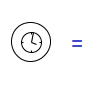
\includegraphics{images/mapping/timer_start.png}
\end{minipage}
\begin{minipage}[c]{0.72\textwidth}
If the expression is a duration:
\begin{lstlisting}[language = Java]
public void execute(){
	while(true){
		[start process]
		try {
			Thread.sleep([time expression]);
		} catch(InterruptedException e) {
		}
	}
}
\end{lstlisting}
If the expression is an exact time:
\begin{lstlisting}[language = Java]
public void execute(){
	try {
			Date then = new SimpleDateFormat("yyyy-MM-dd'T'HH:mm:ss.SSSZ").parse("2011-11-04T10:00:00.000+0100");
			long toSleep = then.getTime() - System.currentTimeMillis();
			if(toSleep>=0){
				try {
					Thread.sleep(toSleep);
				} catch(InterruptedException e) {
				}
				[start process]
			}
		} catch(ParseException e) {
			System.out.println("ParseException: Time has to be in yyyy-MM-dd'T'HH:mm:ss.SSSZ form");
			e.printStackTrace();
		}
}
\end{lstlisting}
\end{minipage}
\caption{Mapping example : Timer Start Event}%
\label{fig:timer_start}%
\end{figure}
\newpage

\textbf{Message}\\
Message Start and End events will influence the signature of the workflow method. The start event defines the parameters and the end event defines it's return type. We can divide message start and end events according to the event's implementation (Service or MessageChannel). 

\textbf{Message with Service implementation}
If the implementation is a Service, the workflow method will be exposed as an action(service). The process will be started by other AgentBean as a service by invoking the exposed action. The signature of the workflow method will be derived from the signature of the implementing service. 
Multiple return type are wrapped in a Serializable array. 

In Figure \ref{fig:message_service} we can see an example mapping of message start and end events with service implementation. The generated workflow method are exposed as an Action with the @Expose code in Line 5. 
\begin{figure}[h]
\begin{minipage}[c]{0.35\textwidth}
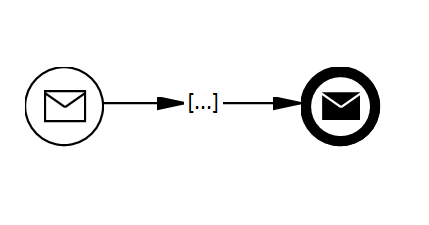
\includegraphics[width=0.9\textwidth]{images/mapping/messageStart.png}
\end{minipage}
\begin{minipage}[c]{0.65\textwidth}
\begin{lstlisting}[language = Java]
public class [Bean-name] extends AbstractMethodExposingBean{
	public final static String ACTION_[workflow name] = "[bean fullname]#[workflow method]"; 
	[...]
	
	@Expose(name = ACTION_[workflow name], scope = ActionScope.GLOBAL)
	public [service output] [workflow method]([service inputs]){
		[...]
		return [service output];
	}
	
	[...]
}
\end{lstlisting}
\end{minipage}
\caption{Mapping example : Message Start and End Events with Service Implementation}%
\label{fig:message_service}
\end{figure}


\newpage
\textbf{Message with MessageChannel implementation}\\
If the implementation is a MessageChannel, an observer will be created and attached to the agent's memory in the \verb|doStart()| method.
The workflow method will get the MessageChannel's payload as a parameter, and it will have no return type (void) and the result will be sent as a message to the specified MessageChannel of the end event. Figure \ref{fig:channel_start} shows a mapping example of a message start event, and in Figure \ref{fig:channel_end}, we can see a mapping example of how a message end event will be mapped.
\begin{figure}[h]
\begin{minipage}[c]{0.28\textwidth}
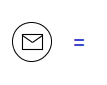
\includegraphics{images/mapping/message_start.png}
\end{minipage}
\begin{minipage}[c]{0.72\textwidth}
\begin{lstlisting}[language = Java]
public class [Bean-name] extends AbstractMethodExposingBean{
	[...]
	
	public void doStart(){
		[...]
		Action joinAction = retrieveAction(ICommunicationBean.ACTION_JOIN_GROUP);
		IGroupAddress groupAddress = CommunicationAddressFactory.createGroupAddress([channel]);
		invoke(joinAction,new Serializable[]{groupAddress});
		SpaceObserver<IFact> [event name or id]_observer = new SpaceObserver<IFact>(){
			public void notify(SpaceEvent<? extends IFact> event) { 
				if(event instanceof WriteCallEvent<?>){ 
					WriteCallEvent<IJiacMessage> wce = (WriteCallEvent<IJiacMessage>) event;
					IJiacMessage message = wce.getObject();
					IFact payload = message.getPayload();
					if(payload!=null && [payload name] instanceof [payload type]&& message.getHeader(IJiacMessage.Header.SEND_TO).equals([channel]){
						memory.remove(message);
						[workflow method](([payload type])payload);
					}
				}
			}
		};
		memory.attach(_nO3bwPwdEeCOWB3dJOsUA_observer);
		[...]
	}
	
	public void [workflow method]([payload type] [payload name]){
		[...]
	}
	
	[...]
}
\end{lstlisting}
\end{minipage}
\caption{Mapping example : Message Start Event with MessageChannel Implementation}%
\label{fig:channel_start}
\end{figure}


\begin{figure}[hbtp]
\begin{minipage}[c]{0.28\textwidth}

\includegraphics{images/mapping/message_end.png}
\end{minipage}
\begin{minipage}[c]{0.72\textwidth}
\begin{lstlisting}[language = Java]
public class [Bean-name] extends AbstractMethodExposingBean{
	[...]
	public void [workflow method]([payload type] [payload name]){
		[...]
		[payload type] [payload name]//payload variable declaration
		[payload name]= new StringOutput("ok");//payload assignment
		Action sendAction = retrieveAction(ICommunicationBean.ACTION_SEND);
		IGroupAddress groupAddress = CommunicationAddressFactory.createGroupAddress([channel]);
		JiacMessage jiacMessage = new JiacMessage([payload name]);
		invoke(sendAction, new Serializable[]{jiacMessage, groupAddress});
	}
	[...]
}
\end{lstlisting}
\end{minipage}
\caption{Mapping example : Message End Event with MessageChannel Implementation}%
\label{fig:channel_end}
\end{figure}
\newpage
\section{Open Issues}

In this chapter, we presented the details of the mapping from BPMN to Jiac AgentBeans. As we can see in some sections, there are some elements that has not been mapped yet. In the future, we will need to study the semantics of the unmapped elements (e.g. multi instance loop, rule events etc.) further and develop their mapping.
	\chapter{Implementation of the transformation}
\label{chap:implementation}
%===============================%
%         Trafo stages          %
%===============================%
In this chapter, we will present the details of the transformation's implementation. We will start with the slightly modified overall transformation structure and then continue with the details of each transformation stages.

\section{Transformation Structure}
As mentioned before in section \ref{sec:vsdt}, the transformation process in the VSDT is divided into 5 stages. We've also mentioned that the default validation and structure mapping provided by the transformation framework are reuseable. For the implementation of the new transformation, the framework's DefaultBpmnValidator and BPMN2StrucBPMNTransformation are being reused, as we can see in Figure \ref{fig:implementation_stages}.

\begin{figure}[h]
	\centering	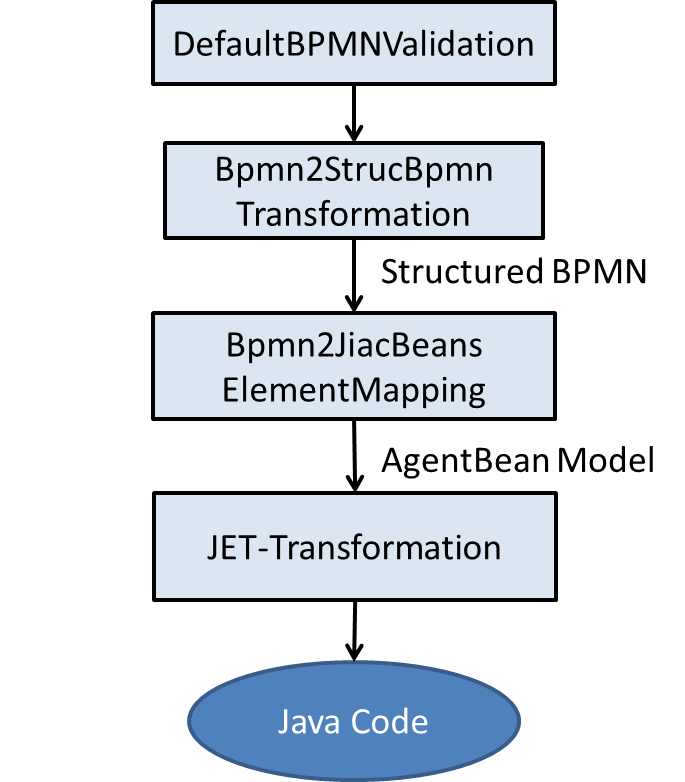
\includegraphics[width=0.5\textwidth]{images/implementation_stages.png}
	\caption{Transformation stages}
	\label{fig:implementation_stages}
\end{figure}

The Element mapping stage is implemented on the basis of the existing Bpmn2JiacV- ElementMapping. It takes a structured Bpmn as a model and transforms each pool contained in the model's business process diagram into a Java object, which represent a model of a java file holding an AgentBean class. For this implementation, a Metamodel of the Jiac AgentBean(see Figure \ref{fig:agentbean_metamodel}) was developed as an intermediate product. 

After all Pools in the business process is completely visited and transformed into AgentBean models, these models are passed over to the JET-Transformation where they will be transformed into a String which represents the content of a Java File. 
\newpage
%===============================%
%       Validation Stage        %
%===============================%
\section{Validation}
The DefaultBPMNValidation is currently used for the validation stage. However, it might be useful that a new validation, that checks whether the expressions given in the model are conform with the Java syntax, to be implemented in the future.

%===============================%
%      Structure Mapping        %
%===============================%
\section{Structure Mapping}
Similar to the validation stage, nothing new was implemented for the structure mapping stage. The default BPMN2StrucBPMN transformation of the VSDT is being reused. In this stage the structure of the process diagram (a directed graph) is being adapted to an equivalent block structure.  

%===============================%
%       Element Mapping         %
%===============================%
\section{Element Mapping}
For the element mapping implementation a visitor based 
%===============================%
%       AgentBean Model         %
%===============================%
\section{AgentBean Model}

An AgentBean model has a list of attributes, methods, action and it may also have some subprocess(because a subprocess is mapped into an inner class of the generated AgentBean).\\\\
For the content of a Method, a Script-Model was also developed. A script is basically a java code element, which can be a single CodeElement(a single line java code), a sequence which contains a list of scripts, or even a block construct such as the while loop, or a try-catch block. 

\begin{figure}[h]
	\centering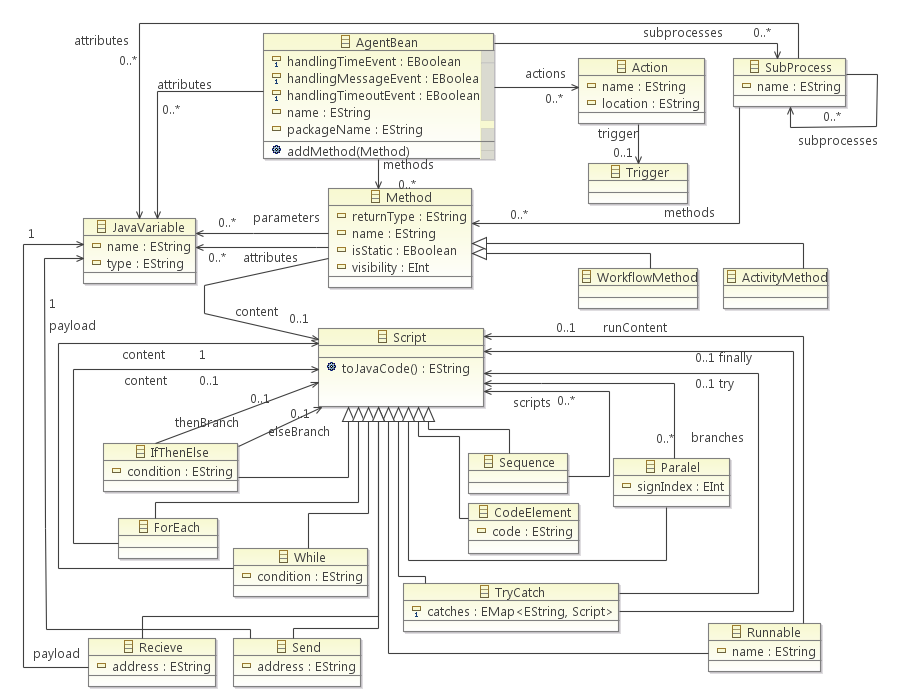
\includegraphics[width=1.0\textwidth]{images/agentBean_metamodel.png}
	\caption{AgentBean - Metamodel}
	\label{fig:agentbean_metamodel}
\end{figure}

Each script implements the method \lstinline[language=Java]{public String toJavaCode()} which returns the java code representation of the script.
In the following listing we can see the implementation of the method in the IfThenElse class:
\begin{lstlisting}[language = Java, caption = toJavaCode() implementation in the IfThenElse class]
	public String toJavaCode() {
		String code = "";
		code += "if("+condition+"){\n";
		if(thenBranch!=null){
			BufferedReader reader = new BufferedReader(new StringReader(thenBranch.toJavaCode()));
			try{
				String line = reader.readLine();
				while(line!=null){
					if(!line.equals("")) code += "\t"+line+"\n";
					line = reader.readLine();
				}
			}catch(IOException e){
				code += "\t//Error occured while reading if branch\n";
			}
		}
		code+="}";
		if(elseBranch!=null){
			code+="else{\n";
			BufferedReader reader = new BufferedReader(new StringReader(elseBranch.toJavaCode()));
			try{
				String line = reader.readLine();
				while(line!=null){
					if(!line.equals("")) code += "\t"+line+"\n";
					line = reader.readLine();
				}
			}catch(IOException e){
				code += "\t//Error occured while reading else branch\n";
			}
			code+="}";
		}
		return code;
	}
\end{lstlisting}

You might notice, that this method is also responsible for the text formatting because this method will be used by the JET-Transformation and the result will then be written in a *.java File. Therefore, as you can see in line 7-11 and 21-25, a tab are added in front of each line in the then and else branch.\\\\
%%%%%%%%%%%%%%%%%%%%%%%%%%%
% Role of MDE             %
%%%%%%%%%%%%%%%%%%%%%%%%%%%
\textbf{The role of MDE in the Implementation}\\\\
The benefits of Model Driven Engineering are also found during the implementation of the AgentBean model. As we can see in Figure \ref{fig:agentbean_metamodel}, it is created graphically using eclipse's Ecore Tools - Ecore Diagramm. With the help of the EMF Generator each element of the model can be easily generated into JavaCode including a Factory class that can be used to instantiate an object of each generated class. This way, we only have to implement the method toJavaCode() for each newly added script, everything else are generated automatically. 


%\newpage
%%%%%%%%%%%%%%%%%%%%%%%%%%%%%%%%%%%%%%%%%%%%%%%%%%%%%%%%%%%%%%%%
%								        JET-Transformation                     %
%%%%%%%%%%%%%%%%%%%%%%%%%%%%%%%%%%%%%%%%%%%%%%%%%%%%%%%%%%%%%%%%
\section{JET-Transformation}
The JET-Transformation consists of 4 Templates( see also Figure \ref{fig:transformation_structure}): 
\begin{enumerate}
	\item agentbeantemplate.javajet
	\item subprocesstemplate.javajet
	\item timeouteventhandler.javajet
	\item timeeventhandler.javajet
	\item messageeventhandler.javajet
\end{enumerate}

\begin{figure}[h]
	\centering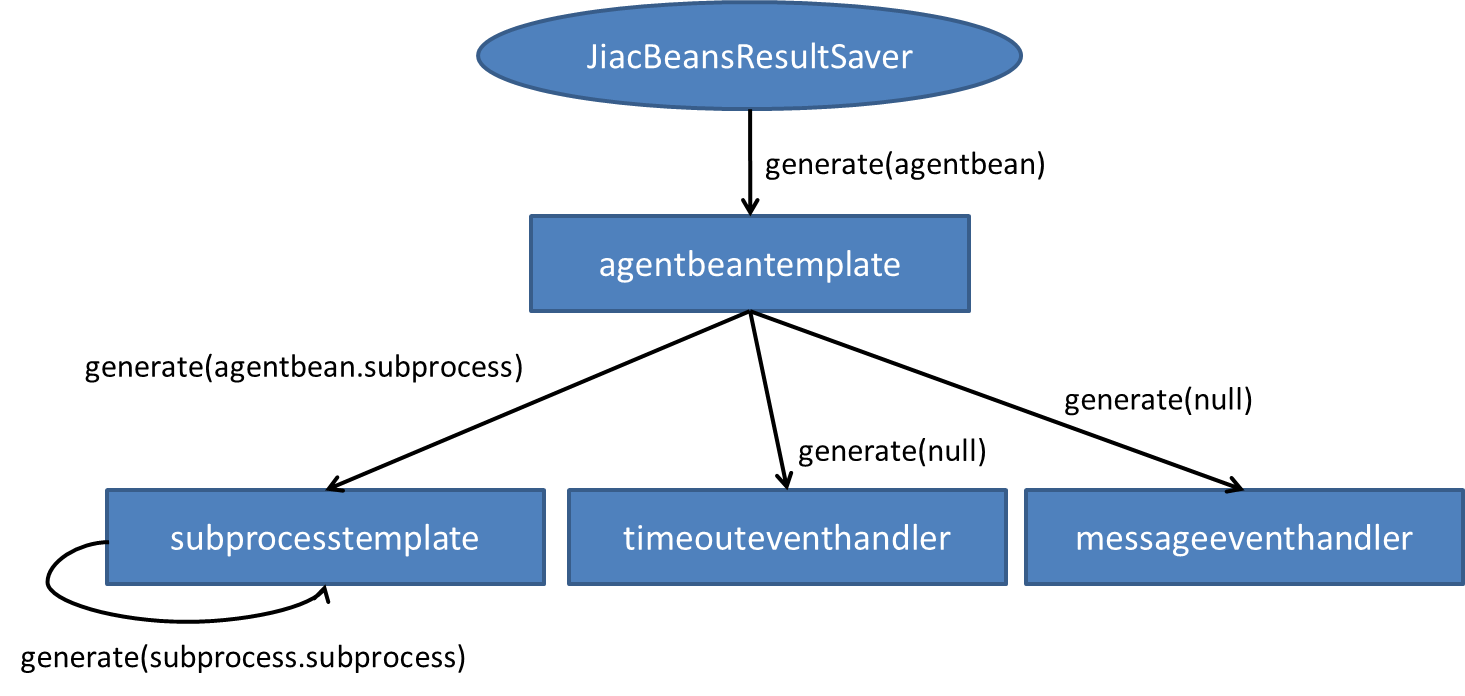
\includegraphics[width=1.0\textwidth]{images/templates_structure.png}
	\caption{JET-Transformation Structure}
	\label{fig:transformation_structure}
\end{figure}

The agentbeantemplate is the main template of the implemented JET-Transformation. An instance of it's Java template class are created by the JiacBeansResultSaver and the generate method will be invoked for each AgentBean model generated in the element mapping stage. 

The subprocesstemplate is invoked by the agentbeantemplate and recursively by the subprocesstemplate itself for each subprocess contained in their argument (an agentbean model or a subprocess model). 

The three handler templates timeouteventhandler, timeeventhandler and messageeventhandler are static templates, which means the result of the generate method does not depend on the argument object. They simply add an inner class TimeoutEventHandler, TimeEventHandler or MessageEventHandler to the AgentBean. They are invoked by the agentbeantemplate if the value of the flag handlingTimeoutEvent or handlingMessageEvent of the agent bean model is true.

\section{Implementation of the Event Handlers}
The Event handlers generated by the above mentioned templates are implemented as an inner class of the generated bean.
They all have a thread as an argument that will be stopped as soon as the expected event is received. The following code listings shows the generated code of the event handlers:

\begin{lstlisting}[language=Java , caption=MessageEventHandler implementation]
class MessageEventHandler extends Thread{
		Thread toStop;
		boolean triggered = false;
		String address;
		Class payloadClass;
		SpaceObserver<IFact> observer;
		Action joinAction;
		Action leaveAction;
		IGroupAddress groupAddress;
		
		public MessageEventHandler(String channel, String payloadType, Thread toStop){
			address = channel;
			this.toStop = toStop;
			joinAction = retrieveAction(ICommunicationBean.ACTION_JOIN_GROUP);
			leaveAction = retrieveAction(ICommunicationBean.ACTION_LEAVE_GROUP);
			groupAddress = CommunicationAddressFactory.createGroupAddress(address);
			try {
				payloadClass = ClassLoader.getSystemClassLoader().loadClass(payloadType);
			} catch (ClassNotFoundException e) {
				log.error("Class "+payloadType+" not Found!");
				e.printStackTrace();
			} 
			observer = new SpaceObserver<IFact>(){
				public void notify(SpaceEvent<? extends IFact> event) {
					if(event instanceof WriteCallEvent<?>){
						Object obj = ((WriteCallEvent) event).getObject();
						if(obj instanceof IJiacMessage){
							IJiacMessage msg = (IJiacMessage)obj;
							if(msg.getHeader(IJiacMessage.Header.SEND_TO).equals(address) &&
							   payloadClass.isInstance(msg.getPayload())){
								memory.remove(msg);
								compensate();
							}
						}
					}
				}
			};		
		}
		
		public void run(){
			invoke(joinAction, new Serializable[]{groupAddress});
			memory.attach(observer);
		}
		
		public void compensate(){
			triggered = true;
			detach();
		}
		
		public void detach(){
			memory.detach(observer);
			invoke(leaveAction, new Serializable[]{groupAddress});
		}
		
		public boolean hasBeenTriggered(){
			return triggered;
		}
}
\end{lstlisting}

\begin{lstlisting}[language=Java , caption=TimeoutEventHandler implementation]
class TimeoutEventHandler extends Thread{
		long timeout;
		Thread toStop;
		boolean triggered = false;
		
		public TimeoutEventHandler(long timeout, Thread toStop){
			this.timeout = timeout;
			this.toStop = toStop;
		}
		
		public void run(){
			try {
				Thread.sleep(timeout);
				triggered = true;
				toStop.stop();
			}catch(InterruptedException e ) { }
		}
		
		public boolean hasBeenTriggered(){
			return triggered;
		}
}
\end{lstlisting}

\begin{lstlisting}[language=Java , caption=TimeEventHandler implementation]
class TimeEventHandler extends Thread{
		Date whenToStop;
		Thread toStop;
		boolean triggered = false;
		
		public TimeEventHandler(String timeExpression, Thread toStop){
			try {
				whenToStop = new SimpleDateFormat("yyyy-MM-dd'T'HH:mm:ss.SSSZ").parse(timeExpression);
			} catch (ParseException e) {
				System.out.println("ParseException: Time Expression has to be in yyyy-MM-dd'T'HH:mm:ss.SSSZ format!");
				e.printStackTrace();
			} 
			this.toStop = toStop;
		}
		
		public void run(){
			long time = whenToStop.getTime();
			while(time>System.currentTimeMillis()){
				try {
					Thread.sleep(100);
				}catch(InterruptedException e ) { }
			}
			toStop.stop();
			triggered = true;
		}
		
		public boolean hasBeenTriggered(){
			return triggered;
		}
}
\end{lstlisting}


Both TimeEventHandler and TimeoutEventHandler are used to handle time events attached to an activity. If the given time expression is a duration, then TimeoutEventHandler will be used. If the given time expression is an exact time, TimeEventHandler will be used. TimeEventHandler parses the given expression into java Date Object using the method \verb|SimpleDateFormat.parse()|, while the TimeoutEventHandler will get a long integer parsed from the time expression. 


%%%%%%%%%%%%%%%%%%%%%%%%%%%%%%%%%%%%%%%%%%%%%%%%%%%%%%%%%%%%%%%%
%           Merging generated and manually edited code         %
%%%%%%%%%%%%%%%%%%%%%%%%%%%%%%%%%%%%%%%%%%%%%%%%%%%%%%%%%%%%%%%%
\section{Merging generated and manually edited code}
The main challenge in generating Java code is how to handle code that has been manually edited. Fortunately, the EMF comes with a solution to this problem : \textbf{JMerge}\cite{JMERGEFAQ}. With JMerge we can...

\subsection{JMerge}
%%%%%%%%%%%%%%%%%%%%%%%%%%%%%%%%%%%%%%%%%%%%%%%%%%%%%%%%%%%%%%%%
%                         Open Issues                          %
%%%%%%%%%%%%%%%%%%%%%%%%%%%%%%%%%%%%%%%%%%%%%%%%%%%%%%%%%%%%%%%%
\section{Open Issues}
implementation not complete


using JET2


better mergerules to mix manually edited and generated code within a method




	\chapter{Example}
\label{chap:examples}

In this chapter we will introduce an example scenario of a process and how the resulting code of the transformation looks like.

\section{The Model}
The example is based on a scenario taken from an actual topic: \textit{electromobility}. The scenario includes a choreography between a MobileApplication, that will be used by a user to reserve a taxi and a number of ETaxi-applications installed in electronic taxis. Figure \ref{fig:usecase} shows the use case model of the \textbf{requestTaxi} process. 
\begin{figure}[h]
	\centering
		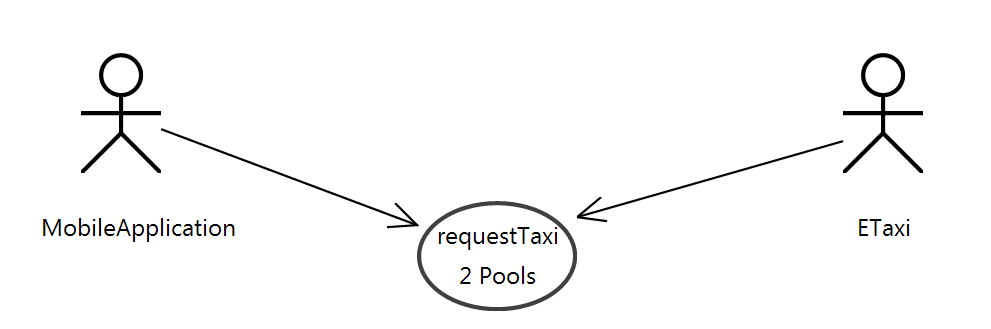
\includegraphics[width=0.8\textwidth]{images/example/usecase.png}
	\label{fig:usecase}
	\caption{Use Case Model}
\end{figure}

In figure \ref{fig:payloads} we can see some data types included in the process which represent the information exchanged in the communication between both pools (the payload of the implementing MessageChannel). The transformation will assume that the classes exist and they will be imported by the generated Agent Bean. Further, because payloads will be wrapped in a JiacMessage, they have to implement the IFact interface.
\begin{figure}[h]
	\centering
		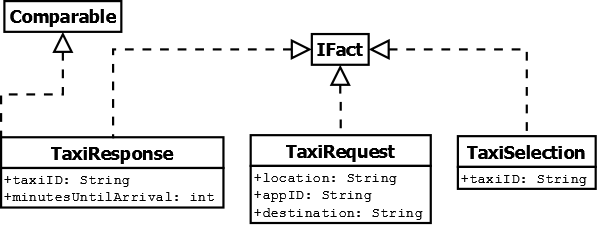
\includegraphics[width=0.8\textwidth]{images/example/payloads.png}
	\label{fig:payloads}
	\caption{Payload data types included in the process diagram}
\end{figure}

\newpage
\subsection{The scenario}
Before we start with the transformation, we will describe the scenario that lies behind the process model shown in figure \ref{fig:example} from the perspective of each pool. 

\textbf{Mobile Application}\\
The process starts with a user requesting a taxi by invoking the service provided by the mobile application. The service will then make a request to all ETaxis by sending information about the user's location, application ID and the destination. Within 30 seconds after sending the request, the mobile application will collect responses from all available ETaxis. Each of these responses contains information about the taxi ID and the estimated time needed by this taxi to arrive at the user's current location. If multiple responses are received, the mobile application will record the best response according to the minimum estimated time. After 30 seconds the application will check whether a response was received. If yes, it will send a notification to all taxis informing which taxi is selected. Then the process will end and the selected taxi's ID will be sent to the user. If no respons is received, it will notify the user that no taxi is currently available. 


\textbf{ETaxi}\\
From the ETaxi perspective, the process starts when a request from a mobile application is received. It will then evaluate the request and decide whether or not the request is interesting e.g according to the distance between the taxi's location and the user's location. If the request is interesting, the ETaxi will then send a response back to the requesting MobileApplication. After that it will wait for a notification from the MobileApplication and check the included taxiID. If the taxiID belongs to the ETaxi, the driver will be informed and the system will navigate to the user's location.


\begin{sidewaysfigure}
	\centering
		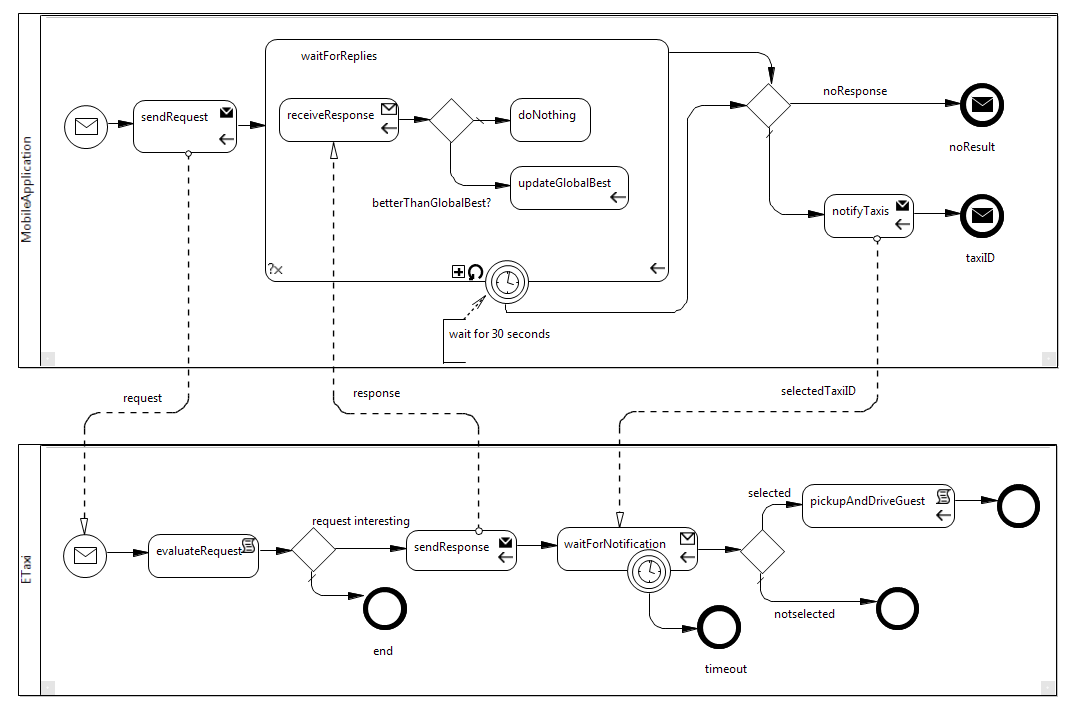
\includegraphics[width = 0.9\textwidth]{images/example/requestTaxi.png}
	\label{fig:example}
	\caption{Business Process Diagram - requestTaxi}
\end{sidewaysfigure}


\subsection{Problem With MessageChannel}
As mentioned in the open issues of the mapping, with the MessageChannel implementation, a message will be broadcasted to all subscribers of a communication group. This is a problem for our scenario since the response from the ETaxis should be sent only to the requesting MobileApplication. In order to keep the scenario as it is, we decided to make a workaround for this problem and create a channel (communication group) where the application ID (appID) is included in the address. This way each mobile application will have its own channel. 

\newpage
At the moment, the implemented element mapping will map the given channel into a String literal (the expression will be wrapped with two quotation marks \verb|"[expression]"|). Obviously we need to avoid the wrapping of the appID variable as a String literal. Therefore we constructed the channel expression as \verb|TaxiResponse-To"+appID+"|. This way the mapped expression will be \verb|"TaxiResponseTo"+appID+""|. Perhaps it would be better if we change the implementation in the future and skip the wrapping of the given expression. Instead we can simply assume that the given expression is a valid Java String literal or a String variable e.g \verb|"TaxiRequest"| or \verb|requestChannel|(requestChannel must be a String variable contained in the Agent Bean).

\section{The Generated Agent Beans}
In this section we will present the Agent Beans generated from the above model. To save space and improve the readability, the generated code will be reduced as follows:
\begin{itemize}
	\item Imports are deleted
	\item Javadoc elements used for JMerge are deleted
	\item The inner class TimeoutEventHandler which we already presented in section \ref{sec:handler} is deleted
	\item Some empty lines are deleted
\end{itemize}
Beside the mentioned reduction, no other changes were made to the generated code. All codes and comments are generated directly from the model.

\textbf{1. MobileApplication\_requestTaxi}\\

\begin{lstlisting}[language=java, caption= Generated Agent Bean - MobileApplication\_requestTaxi]
package mobileapplication;
[imports]
public class MobileApplication_requestTaxi extends AbstractMethodExposingBean{
	public final static String ACTION_REQUESTTAXI = "mobileapplication.MobileApplication_requestTaxi#requestTaxi"; 
	
	TaxiResponse globalBest;
	boolean noResponse;
	String appID;
	String location;
	String destination;
	
	@Expose(name = ACTION_REQUESTTAXI, scope = ActionScope.GLOBAL)
	public String requestTaxi(String currentLocation, String currentDestination) {
		location= currentLocation;
		destination= currentDestination;
		sendRequest();
		Thread waitForReplies = new Thread(new Runnable(){
			public void run(){
				WaitForRepliesSubProcess waitForReplies = new WaitForRepliesSubProcess();
				waitForReplies.run();
			}
		});
		TimeoutEventHandler wait30Seconds_TimeoutHandler = new TimeoutEventHandler(30000,waitForReplies);
		waitForReplies.start();
		wait30Seconds_TimeoutHandler.start();
		try {
			waitForReplies.join();
			wait30Seconds_TimeoutHandler.stop();
		} catch(InterruptedException e) {
		}
		
		if(noResponse){
			String taxiID;
			taxiID= "none available";
			return taxiID;
		} else {
			notifyTaxis();
			String taxiID;
			taxiID= globalBest.getTaxiID();
			return taxiID;
		}
	}

	private void sendRequest() {
		TaxiRequest request;
		request= new TaxiRequest(location,appID,destination);
		Action sendAction = retrieveAction(ICommunicationBean.ACTION_SEND);
		IGroupAddress groupAddress = CommunicationAddressFactory.createGroupAddress("TaxiRequest");
		JiacMessage jiacMessage = new JiacMessage(request);
		invoke(sendAction, new Serializable[]{jiacMessage, groupAddress});
	}

	private void notifyTaxis() {
		SelectedTaxi selectedTaxi;
		selectedTaxi= new SelectedTaxi(globalBest.getTaxiID());
		Action sendAction = retrieveAction(ICommunicationBean.ACTION_SEND);
		IGroupAddress groupAddress = CommunicationAddressFactory.createGroupAddress("notification");
		JiacMessage jiacMessage = new JiacMessage(selectedTaxi);
		invoke(sendAction, new Serializable[]{jiacMessage, groupAddress});
	}

	class WaitForRepliesSubProcess{
		
		TaxiResponse currentResponse;
		
		public void run() {
			noResponse= true;
			while(true) {
				receiveResponse();
				if(currentResponse.compareTo(globalBest)>0){
					updateGlobalBest();
				} else {
					doNothing();
				}
			}
		}
	 
		private void receiveResponse() {
			Action joinAction = retrieveAction(ICommunicationBean.ACTION_JOIN_GROUP);
			Action leaveAction = retrieveAction(ICommunicationBean.ACTION_LEAVE_GROUP);
			IGroupAddress groupAddress = CommunicationAddressFactory.createGroupAddress("TaxiResponseTo"+appID+"");
			invoke(joinAction,new Serializable[]{groupAddress});
			TaxiResponse response = null;
			while(response==null) {
				Set<IFact> all = memory.readAll();
				for(IFact fact : all){
					if(fact instanceof JiacMessage) {
						JiacMessage jiacMessage = (JiacMessage)fact;
						if(jiacMessage.getPayload() instanceof TaxiResponse && jiacMessage.getHeader(IJiacMessage.Header.SEND_TO).equals("TaxiResponseTo"+appID+"")) {
							memory.remove(jiacMessage);
							response = (TaxiResponse) jiacMessage.getPayload();
							break;
						}
					}
				}
				try{
					Thread.sleep(100);
				} catch(InterruptedException e) { }
			}
			invoke(leaveAction, new Serializable[]{groupAddress});
			noResponse= false;
			currentResponse= response;
		}
	 
		private void doNothing() {
		}
	 
		private void updateGlobalBest() {
			globalBest= currentResponse;
		} 
	}
}
\end{lstlisting}

In the MobileApplication\_requestTaxi Bean, almost every logic is generated from the model. The workflow method requestTaxi is exposed as an action. All methods are filled with needed operations e.g. the decision whether the currentResponse is better than the globalBest is made by using the compareTo method of the TaxiResponse class. There is only one small yet fatal aspect missing in the generated code. You might notice that while other variables are initialized somewhere in the assignment of a method, the initialization of the appID variable can't be found in the generated code. To ensure that each instance of the MobileApplication\_requestTaxi has a unique ID, the initialization cannot be included in the model. We have to e.g. add a constructor and implement the initialization of the appID in it to make the code works completely. This problem also exists in the generated ETaxi\_requestTaxi code.

\textbf{2. ETaxi\_requestTaxi}\\

\begin{lstlisting}[language=java, caption= Generated Agent Bean - ETaxi\_requestTaxi]
package etaxi;
[imports]
public class ETaxi_requestTaxi extends AbstractMethodExposingBean{
	public final static String ACTION_REQUESTTAXI = "etaxi.ETaxi_requestTaxi#requestTaxi"; 

	boolean requestInteresting;
	String taxiID;
	String globalLocation;
	int estimatedTime;
	String appID;
	TaxiRequest currentRequest;
	SelectedTaxi selection;
	boolean available;

	@Expose(name = ACTION_REQUESTTAXI, scope = ActionScope.GLOBAL)
	public void requestTaxi(TaxiRequest request) {
		currentRequest= request;
		evaluateRequest();
		if(requestInteresting){
			sendResponse();
			Thread waitForNotification = new Thread(new Runnable(){
				public void run(){
					waitForNotification();
				}
			});
			TimeoutEventHandler _x5RCUAGWEeGC8PuSIWxlmQ_TimeoutHandler = new TimeoutEventHandler(60000,waitForNotification);
			waitForNotification.start();
			_x5RCUAGWEeGC8PuSIWxlmQ_TimeoutHandler.start();
			try {
				waitForNotification.join();
				_x5RCUAGWEeGC8PuSIWxlmQ_TimeoutHandler.stop();
			} catch(InterruptedException e) {
			}
			if(!_x5RCUAGWEeGC8PuSIWxlmQ_TimeoutHandler.hasBeenTriggered()){
				if(selection.getTaxiID().equals(taxiID)){
					pickupAndDriveGuest();
				} else {
				}
			}
		} else {
		}
	}

	public void doStart() {
		Action joinAction = retrieveAction(ICommunicationBean.ACTION_JOIN_GROUP);
		IGroupAddress groupAddress = CommunicationAddressFactory.createGroupAddress("TaxiRequest");
		invoke(joinAction,new Serializable[]{groupAddress});
		SpaceObserver<IFact> _B8QyYAF3EeGC8PuSIWxlmQ_observer = new SpaceObserver<IFact>(){
			public void notify(SpaceEvent<? extends IFact> event) { 
				if(event instanceof WriteCallEvent){ 
					Object obj  = ((WriteCallEvent) event).getObject();
					if (obj instanceof IJiacMessage){
						IJiacMessage message = (IJiacMessage)obj;
						IFact payload = message.getPayload();
						if(payload!=null && payload instanceof TaxiRequest&& message.getHeader(IJiacMessage.Header.SEND_TO).equalsIgnoreCase("TaxiRequest")){
							memory.remove(message);
							requestTaxi((TaxiRequest)payload);
						}
					}
				}
			}
		};
		memory.attach(_B8QyYAF3EeGC8PuSIWxlmQ_observer);
	}

	private void evaluateRequest() {
		//script activity
		//TODO implement code 
		requestInteresting = true; //every request is interesting
	}

	private void sendResponse() {
		TaxiResponse response;
		response= new TaxiResponse(taxiID, estimatedTime);
		Action sendAction = retrieveAction(ICommunicationBean.ACTION_SEND);
		IGroupAddress groupAddress = CommunicationAddressFactory.createGroupAddress("TaxiResponseTo"+appID+"");
		JiacMessage jiacMessage = new JiacMessage(response);
		invoke(sendAction, new Serializable[]{jiacMessage, groupAddress});
	}

	private void waitForNotification() {
		Action joinAction = retrieveAction(ICommunicationBean.ACTION_JOIN_GROUP);
		Action leaveAction = retrieveAction(ICommunicationBean.ACTION_LEAVE_GROUP);
		IGroupAddress groupAddress = CommunicationAddressFactory.createGroupAddress("notification");
		invoke(joinAction,new Serializable[]{groupAddress});
		SelectedTaxi selectedTaxi = null;
		while(selectedTaxi==null) {
			Set<IFact> all = memory.readAll();
			for(IFact fact : all){
				if(fact instanceof JiacMessage) {
					JiacMessage jiacMessage = (JiacMessage)fact;
					if(jiacMessage.getPayload() instanceof SelectedTaxi && jiacMessage.getHeader(IJiacMessage.Header.SEND_TO).equals("notification")) {
						memory.remove(jiacMessage);
						selectedTaxi = (SelectedTaxi) jiacMessage.getPayload();
						break;
					}
				}
			}
			try{
				Thread.sleep(100);
			} catch(InterruptedException e) { }
		}
		invoke(leaveAction, new Serializable[]{groupAddress});
		selection= selectedTaxi;
	}

	private void pickupAndDriveGuest() {
		available= false;
		// TODO add code to navigate to guest's location
		available= true;
	}
	
}
\end{lstlisting}

Similar to the MobileApplication\_requestTaxi Bean, the initialization of the taxiID is also missing in the generated code. Moreover, unlike the MobileApplication\_request-Taxi Agent Bean, we did not include all the logic in the model (e.g. for evaluating whether a request is interesting). By this we showed that the quantity of the generated code might vary depending on how we design the model.


In this chapter we have presented an example of the transformation in which some problems regarding the current mapping and transformation are shown. We have also shown how agents can be designed and created easily by modeling a business process. 

	\chapter{Conclusion}
% Benefits of MDD in product and in the implementation

%%%%%%%%%%%%%%%%%%%%%%%
%Future work          %
%%%%%%%%%%%%%%%%%%%%%%%

%- Mapping not complete

%- JET2?

%- Better Merging with JMerges
 

	
	\begin{appendix}
		% Kapitel in diesem Bereicht erscheinen als Anhänge
	\end{appendix}
	\nocite{*}
	\newpage
	\bibliographystyle{plain}
	\bibliography{bibliography}
	\addcontentsline{toc}{chapter}{\bibname}
	
\end{document}

